\documentclass[11pt]{article}
\usepackage[margin=1in]{geometry}
\usepackage{amsmath,amssymb,booktabs,caption,graphicx,natbib,pdflscape,setspace}
\usepackage{url}
\urlstyle{same}
\onehalfspacing
\newtheorem{proposition}{Proposition}
\newtheorem{lemma}{Lemma}
\newtheorem{corollary}{Corollary}
\newcommand{\figurenotes}[2]{\begin{minipage}{0.96\linewidth}\small\textit{Source:} #1\par\textit{Notes:} #2\end{minipage}}
\title{Before the Levy: Beef Prices During Denmark's Cattle-Policy Transition}
\author{Diego Gonz\'alez-Gonz\'alez}
\date{24 September 2026}

\begin{document}
\maketitle

\begin{abstract}
Can announcements of future environmental charges affect markets before collection begins? I examine beef prices around Denmark's 2024 cattle-policy agreements. A model with costly adjustment of production plans predicts an anticipatory price increase, but the empirical comparisons do not isolate that mechanism. Beef rose by 0.064 log points relative to other Danish foods after June 2024; almost all of this average contrast arose in 2025, and its conventional significance depends on the serial-correlation bandwidth. Relative to beef prices in other EU countries, the estimate is 0.016 log points (standard error 0.029). Slaughter responses are imprecise. The grocery source records price changes without a historical availability panel, so its event-price comparison cannot independently validate a monthly posted-price effect. A contemporaneous change in cattle manure regulation further prevents attribution to the future emissions tax alone. The evidence describes a cattle-policy episode with substantial counterfactual and mechanism uncertainty.
\end{abstract}
\noindent\textbf{JEL codes:} H23, Q18, Q54, Q58.\par
\noindent\textbf{Keywords:} Environmental taxation; policy announcements; anticipation; beef prices; livestock production; synthetic difference-in-differences.


\section{Introduction}
Environmental policy can change economic decisions well before it changes firms' current tax liabilities. Producers expecting a future emissions charge may revise investment, procurement, and output plans when the policy is announced. Consumers may then face different prices during the years that separate agreement from implementation. Understanding this interval matters for the evaluation of climate policy: estimates beginning with the first tax payment can miss part of the adjustment that the policy has already induced.

I study beef-market outcomes during Denmark's 2024 cattle-policy transition and ask whether their timing and magnitude can be reconciled with anticipation of a future emissions charge. The theoretical starting point is a competitive industry in which changing production plans is costly. A credible increase in expected future charges reduces the profitability of output at implementation. Linked production decisions can then bring some adjustment forward. A model in which producers instead allocate a fixed stock between current and future slaughter gives the opposite price prediction. These mechanisms motivate examining both prices and slaughter, while leaving their relative importance an empirical question.

Denmark's Green Tripartite agreement provides the setting. On 24 June 2024, the government and negotiating parties agreed to introduce a tax on livestock greenhouse-gas emissions from 2030 \citep{danishgovernment2024}. The expected liability was not necessarily entirely new information: an expert group had published agricultural carbon-tax models in February, and a parliamentary implementation agreement followed in November \citep{danishexpert2024,danishimplementation2024}. Beef is the focus because cattle production involves substantial emissions and biological adjustment lags \citep{rosen1994}. The April announcement and July end of the cattle nitrate derogation create a separate, overlapping cost shock \citep{danishnitrates2024}. Accordingly, the empirical post indicator describes this policy episode; it cannot identify the isolated effect of the June emissions-tax news.

I use Statistics Denmark's monthly consumer price indices to compare beef with other, unexposed Danish foods. This difference-in-differences (DiD) contrast is 0.064 log points, but it is concentrated in 2025 and is sensitive to the serial-correlation adjustment. A second comparison uses Eurostat's harmonized beef-and-veal index for Denmark and the other EU countries. Its synthetic-DiD estimate is 0.016 log points with a 0.029 standard error. This comparison addresses common European beef shocks more directly, although it too cannot separate the two Danish cattle policies. Grocery price histories provide useful product descriptions and a provisional level benchmark, but their entries are changes in quoted prices rather than verified daily observations. Historical product availability cannot be recovered from the frozen snapshot, so I do not interpret its event-price regression as corroborating evidence on monthly posted prices.

To examine the production margin, I use official monthly bovine slaughter statistics. Denmark is compared with 26 other EU countries, all measured in the same commodity and units. The main synthetic-DiD estimate for slaughter weight is $-0.066$ log units, with a wide interval. The estimate is close to zero with a longer, seasonally adjusted pre-period. Counts of slaughtered cattle provide similarly imprecise evidence. These results leave a substantial range of production responses compatible with the data and qualify the interpretation of the positive price estimates.

Identification also requires attention to other changes in the Danish cattle sector. In April 2024, the government announced that the cattle derogation from the EU Nitrates Directive would end on 31 July 2024, increasing costs for some cattle farms \citep{danishnitrates2024}. This change overlaps the post-announcement period and can affect the same outcomes as the emissions-tax news. Cross-country comparisons help account for common beef-market developments, but cannot separate these two Danish policy changes. I therefore interpret the estimates as evidence around the announcement episode, conditional on the stated comparison assumptions.

The price evidence raises a quantitative question about the model. Under stationary two-date primitives, even full adjustment cannot raise the model price by more than a discounted fraction of the expected future output wedge. Applying the paper's broad lifecycle-emissions benchmark to the average announced output burden yields a smaller bound than the DKK/kg equivalent of the preferred within-Denmark price contrast. This tension is conditional on an imperfect grocery level anchor, an unverified causal share of the contrast, and a stylized two-date model; it does not reject anticipation. I use a separate social-cost-of-carbon (SCC) comparison only to show how these assumptions change hypothetical price magnitudes, without interpreting consumer prices as internalized damages.

The analysis relates to anticipation of environmental regulation \citep{smulders2012,rittenhouse2018} and transmission of emissions costs into product prices \citep{fabra2014}. It uses the model to specify what a price response would require, then shows how different counterfactuals and observed timing constrain that interpretation. Section~\ref{sec:theory} develops the model. Sections~\ref{sec:data} and \ref{sec:identification} describe measurement and comparisons. Section~\ref{sec:results} presents price and slaughter evidence. Section~\ref{sec:calibration} gives conditional price accounting; Sections~\ref{sec:discussion} and \ref{sec:conclusion} discuss the remaining identification limits.

\section{Theoretical Framework}\label{sec:theory}
\subsection{A credible future tax and planned supply}
There are two decision dates: the announcement date, normalized to $0$, and the implementation date $T>0$. Let $Q_t>0$ denote aggregate beef output at date $t\in\{0,T\}$, let $P_t(Q_t)$ be inverse demand with $P_t'(Q_t)<0$, and let $C_t(Q_t)$ be the industry's private production cost with $C_t'(Q_t)>0$ and $C_t''(Q_t)\geq0$ for $Q_t>0$. For an arbitrary reference quantity $\bar Q_t>0$, define the competitive-market potential net of production cost as
\begin{equation}
G_t(Q)\equiv\int_{\bar Q_t}^Q P_t(x)\,dx-C_t(Q).
\end{equation}
The reference quantity changes only an additive constant. Thus $G_t'(Q)=P_t(Q)-C_t'(Q)$ and $G_t''(Q)=P_t'(Q)-C_t''(Q)<0$. One unit of output generates $\chi>0$ tons of CO2-equivalent emissions. The statutory tax at $T$ is $\tau_T$ DKK per ton of CO2e. Under risk neutrality, the announcement creates the expected output wedge
\begin{equation}
\omega\equiv\chi E_0[\tau_T],
\qquad E_0[\tau_T]=\pi\tau
\end{equation}
in the special case in which the tax equals $\tau>0$ with implementation probability $\pi\in[0,1]$ and zero otherwise. Here $E_0[\cdot]$ is the expectation conditional on information at announcement. The implementation-date output plan is committed before implementation uncertainty is resolved and cannot be conditioned on the realization of $\tau_T$. Expected tax payments are therefore $\chi E_0[\tau_T]Q_T$.

Production planning is intertemporal. Changing planned output between dates costs $\kappa(Q_T-Q_0)^2/2$, where $\kappa\geq0$ summarizes biological lags, capacity adjustment, and procurement commitments. Let $\beta\in(0,1]$ be the one-period discount factor and $\delta\equiv\beta^T$ the discount factor from announcement to implementation. Assume an interior maximizer exists. Because the following potential is strictly concave, that maximizer is unique:
\begin{equation}\label{eq:potential}
G_0(Q_0)+\delta\left[G_T(Q_T)-\omega Q_T-
\frac{\kappa}{2}(Q_T-Q_0)^2\right].
\end{equation}
The potential is a device for representing competitive equilibrium. Firms take prices as given, and the first-order conditions equate those prices to private marginal production and adjustment costs. This interpretation assumes that the aggregate cost and adjustment schedules represent the industry's feasible allocation across firms. Here $Q_t$ denotes planned market output, and $\kappa$ summarizes the connection between plans across dates. The model abstracts from detailed herd accounting and foreign supply. Applying its price prediction to Danish retail markets consequently also requires that trade and distribution margins do not fully offset the domestic response.

\begin{proposition}[Anticipatory contraction]\label{prop:anticipation}
Suppose the solution to \eqref{eq:potential} is interior and $\kappa>0$. A larger expected implementation wedge reduces planned output both before and at implementation and raises the announcement-period market price:
\begin{equation}
\frac{\partial Q_0}{\partial\omega}<0,
\qquad
\frac{\partial Q_T}{\partial\omega}<0,
\qquad
\frac{\partial P_0}{\partial\omega}>0.
\end{equation}
The policy-induced level change is zero when the policy is not credible ($\pi=0$). The marginal pre-implementation response is zero when adjustment is costless ($\kappa=0$). With fixed adjustment curvature and demand and cost curvatures bounded away from zero, it converges to zero as implementation becomes arbitrarily distant ($T\rightarrow\infty$) when $\beta<1$.
\end{proposition}

The proof is in Appendix~\ref{app:theory}. To derive demand and supply from primitives, suppose preferences and technology are stationary across the two dates. A representative household consumes beef $q_t>0$ and a numeraire good $z_t$. Its quasi-linear utility is
\begin{equation}\label{eq:utility}
u(z_t,q_t)=z_t+
\begin{cases}
A\,q_t^{1-1/\varepsilon}/(1-1/\varepsilon),&\varepsilon\neq1,\\
A\log q_t,&\varepsilon=1,
\end{cases}
\end{equation}
where $A>0$ is the taste shifter and $\varepsilon>0$ is the absolute price elasticity of beef demand. The numeraire price is one and income is sufficient for an interior solution. Utility maximization subject to $z_t+p_tq_t\leq y_t$, where $p_t$ is the beef price and $y_t$ is income, followed by market clearing $q_t=Q_t$, gives inverse demand
\begin{equation}\label{eq:isoelastic_demand}
P(Q)=A Q^{-1/\varepsilon}.
\end{equation}
Quasi-linearity isolates the commodity-market channel from income effects; it is not required for Proposition~\ref{prop:anticipation}. The isoelastic schedule is interpreted locally around $Q^*>0$, rather than as a literal description of willingness to pay near zero consumption.

On the production side, let a representative competitive producer use fixed capital $K>0$ and a variable composite input $X_t\geq0$ to produce
\begin{equation}\label{eq:cobb_douglas}
Q_t=B K^{1-\alpha}X_t^{\alpha},
\qquad B>0,\quad \alpha\in(0,1),
\end{equation}
where $B$ is total factor productivity and $\alpha$ is the output elasticity of the variable input. If that input costs $v>0$ per unit, conditional cost minimization gives
\begin{equation}\label{eq:micro_cost}
C(Q)=v\left(\frac{Q}{BK^{1-\alpha}}\right)^{1/\alpha},
\qquad C'(Q)=mQ^{\eta},
\end{equation}
where $\eta\equiv(1-\alpha)/\alpha>0$ is the inverse supply elasticity and $m\equiv(v/\alpha)(BK^{1-\alpha})^{-1/\alpha}>0$. Here $K$ is quasi-fixed sectoral productive capacity: entry and major capacity expansion are suppressed over the model horizon. The function $C(Q_t)$ captures within-date variable cost conditional on that capacity, whereas $\kappa(Q_T-Q_0)^2/2$ captures additional dynamic reconfiguration costs not contained in $X_t$. Fixed capacity makes variable cost strictly convex. The no-tax, no-adjustment static equilibrium therefore has
\begin{equation}\label{eq:baseline_equilibrium}
Q^*=\left(\frac{A}{m}\right)^{1/(\eta+1/\varepsilon)},
\qquad P^*=A(Q^*)^{-1/\varepsilon}=m(Q^*)^{\eta}.
\end{equation}

\begin{corollary}[Microfounded local incidence]\label{cor:microfoundation}
Under \eqref{eq:utility}--\eqref{eq:micro_cost} and $\kappa>0$, define $s\equiv\eta+1/\varepsilon>0$, the normalized adjustment curvature $\rho\equiv\kappa Q^*/P^*>0$, and the normalized expected wedge $\widehat{\omega}\equiv\omega/P^*$. At the stationary zero-wedge equilibrium $Q_0=Q_T=Q^*$, the exact local comparative statics are
\begin{align}
\left.\frac{\partial\log Q_0}{\partial\widehat{\omega}}\right|_{\widehat{\omega}=0}
&=-\frac{\delta\rho}{s[s+\rho(1+\delta)]},\label{eq:micro_q0}\\
\left.\frac{\partial\log Q_T}{\partial\widehat{\omega}}\right|_{\widehat{\omega}=0}
&=-\frac{s+\delta\rho}{s[s+\rho(1+\delta)]},\label{eq:micro_qt}\\
\left.\frac{\partial\log P_0}{\partial\widehat{\omega}}\right|_{\widehat{\omega}=0}
&=\frac{\delta\rho}{\varepsilon s[s+\rho(1+\delta)]}>0.\label{eq:micro_price}
\end{align}
\end{corollary}

Appendix~\ref{app:theory} derives the corollary. Equation~\eqref{eq:micro_price} is exact for a marginal wedge around the untaxed stationary equilibrium; finite changes obtained from it are first-order approximations, not global effects. Since $\omega=\pi\tau\chi$, the exact marginal response to the announced rate at $\tau=0$ equals the coefficient in \eqref{eq:micro_price} times $\pi\chi/P^*$. Its local marginal magnitude increases with credibility $\pi$, emissions intensity $\chi$, proximity to implementation $\delta$, and adjustment curvature $\rho$. Technology curvature and demand curvature determine the quantity response through $s$; $1/\varepsilon$ additionally maps the output response into the price response. The result does not imply that the observed retail-price change equals the future tax wedge.

\begin{corollary}[Two-date price bound]\label{cor:price_bound}
Under stationary demand and costs, weakly increasing marginal production cost, an interior solution, and $\omega>0$, the finite announcement-date response satisfies
\begin{equation}\label{eq:price_bound}
P_0-P^*\leq\frac{\delta}{1+\delta}\omega.
\end{equation}
The bound concerns the model's market price and expected output wedge; it is not a bound on an observed retail-price change in an open, multi-period economy.
\end{corollary}
The proof is in Appendix~\ref{app:theory}. The bound gives the model a quantitative implication: for $\delta\leq1$, the announcement price response cannot exceed one half of the anticipated future output wedge under these assumptions.

\subsection{From planned output to measured beef markets}
The two-date $Q_t$ suppresses several livestock margins. A stock-flow representation makes the distinction explicit. If $H_t$ is the cattle stock, $B_t$ births or additions, $S_t$ slaughtered animals, $\mu$ other attrition, and $w_t$ mean carcass weight, then
\begin{equation}\label{eq:herd_accounting}
H_{t+1}=(1-\mu)H_t+B_t-S_t,\qquad Q_t=w_tS_t.
\end{equation}
Domestic beef consumption can differ from $Q_t$ through imports, exports, and inventory changes. Its retail price can differ from the domestic producer price through processing and distribution margins. Equation~\eqref{eq:herd_accounting} shows why an initial herd-retention response could lower slaughter counts before changing carcass weight, and why an import response could attenuate the retail price effect. Dairy co-production makes births and retention depend on dairy-market conditions as well. The available data observe slaughter weight and heads but do not identify all of these flows or margins.

For an animal with taxable emissions $e_i$ and deduction $d_i$, a simplified liability is $\tau\max\{e_i-d_i,0\}$. Where $e_i>d_i$, the marginal incentive to reduce taxable emissions is $\tau$, whereas the average liability per unit of output is $\tau(e_i-d_i)/q_i$ for output $q_i$. The two-date $\omega$ is closer to the latter on a fixed-intensity output margin. Gross lifecycle emissions can enter damages without equaling net taxable farm emissions. These distinctions prevent the model's single $\chi$ from being used simultaneously as a measured damage intensity and a measured tax base.

\subsection{Environmental benchmark and a sign-reversing boundary case}
Let environmental damages at date $t$ be $D_t(E_t)$, where emissions are $E_t=\chi Q_t$, $D_t'(E_t)>0$, and $D_t$ is measured in DKK. Define $MD_t^e\equiv D_t'(E_t)$ as marginal damage per ton of CO2e. The standard Pigouvian benchmark is
\begin{equation}\label{eq:pigou}
\tau_t^P=MD_t^e.
\end{equation}
For the paper's accounting exercise, I set $MD_t^e=SCC_t$ under an explicit one-for-one valuation of a ton of CO2e at the CO2 SCC. This convention is not a mechanical equivalence for methane and nitrous oxide merely because global-warming potentials express them in CO2e.

\begin{proposition}[Local welfare effect]\label{prop:welfare}
Suppose tax revenue is rebated lump-sum, administration is costless, private and social discount factors coincide, emissions intensity is fixed, adjustment costs are real resource costs, and the assumptions of Proposition~\ref{prop:anticipation} hold. Starting from no emissions price, a small increase in a credible future tax raises welfare whenever marginal environmental damage is positive. More generally, an increase in $\omega$ raises welfare locally if the expected output wedge does not exceed marginal implementation-date damage per unit of output, $\omega\leq\chi D_T'(E_T)$; the induced pre-implementation contraction supplies an additional benefit when $D_0'(E_0)>0$.
\end{proposition}

The welfare result concerns a marginal policy change from an initially unpriced externality under the model's assumptions. Assessing the Danish rate requires a further distinction between output and emissions-intensity choices. The announced 2030 schedule has a DKK 300/tCO2e marginal abatement incentive, while the per-animal deduction produces a DKK 120/tCO2e average burden at the reference emissions intensity. Both amounts are stated in 2022 prices \citep{danishgovernment2024,danishtaxministry2024}. For a representative animal with fixed reference intensity, the latter provides the closer approximation to the model's output wedge. Farms with different emissions per animal face different average burdens.

Finally, the sign in Proposition~\ref{prop:anticipation} is not mechanical. Suppose instead that a fixed stock $\mathcal S>0$ of slaughterable output, measured in the same units as $Q_t$, must be allocated across the two dates, so $Q_0+Q_T=\mathcal S$, with an interior allocation $0<Q_0<\mathcal S$ and no margin for planned herd contraction. If the tax liability applies to later slaughtered output, a future tax makes later slaughter relatively less attractive, shifts slaughter to date 0, and therefore gives $\partial Q_0/\partial\omega>0$ and $\partial P_0/\partial\omega<0$. This pure reallocation result need not apply if emissions accrue continuously before slaughter. The preemptive-slaughter channel is the livestock analogue of an anticipation or green-paradox response \citep{smulders2012}. A positive price response is compatible with planned contraction. The slaughter estimates below examine its quantity implication, while allowing for the distinct timing mechanism in the fixed-stock model.

\section{Data and Panel Construction}\label{sec:data}
\subsection{Scraped grocery-price microdata}
The grocery source is the historical catalog assembled by dagligepriser.dk. Its collector checks prices daily, but the retained history adds an entry when the price, quantity, or unit changes; unchanged daily quotes do not create entries. The available June 2026 snapshot also lacks a historical availability record for every store and product. I therefore cannot distinguish a continuing unchanged price from an intervening exit or failed collection. Averaging entries within a product--store--month measures the average of recorded change events, not the time-weighted price paid during that month. A month with no change can disappear even if the product was continuously sold. The resulting regression is retained as a diagnostic of the event records and is not used as independent evidence on monthly posted prices. A validated price-spell panel would require dated availability or archived daily snapshots.

Prices are converted to DKK per kilogram for mass units and DKK per litre for volume units. Reported package quantities take precedence. When quantity or unit fields are absent, the procedure searches the product description for a number followed by kg, g, litre, ml, or cl. Grams, millilitres, and centilitres are converted to their base units before dividing price by quantity. Items measured only per piece and observations with missing, non-positive, or unsupported quantities are excluded. Because normalized prices remain right-skewed, estimation uses their natural logarithm and Table~\ref{tab:descriptives} reports medians and quartiles as well as means.

Candidate beef names are initially found with Danish and English meat terms, then screened against the public product descriptions using a six-category Jev classification and a conservative core-beef probability threshold. I inspected the retained names and excluded evident false positives such as beef-flavored noodles and sliced prepared beef. This is a reproducible screening rule, not an externally validated measure of classifier precision. Prepared dishes, plant substitutes, pet food, mixed livestock products, and uncertain candidate names are excluded. Livestock-exposed food products, including poultry, eggs, and dairy, are excluded from the control group. Package parsing now recognizes multipacks such as two 400 g units; reported mass or volume remains the first source for normalization. A classification audit cannot repair the absence of historical price spells or availability.

The event month, June 2024, is excluded from the grocery pre- and post-periods. The window is October 2023--September 2025, excluding June, and calendar event time retains an empty slot at zero; May is $-1$ and July is $+1$. The end date precedes the officially dated October 2025 bovine viral diarrhoea outbreak, although surveillance detected an affected dairy herd in September \citep{dvfaBVD,dvt2025}. That endpoint does not rule out earlier market responses to the disease.

Among 151 screened beef product--store pairs with a recorded event on both sides of the announcement, events appear in 1,105 of 2,552 months between each pair's first and last record, excluding June 2024 (43.3 percent). The corresponding share among 13,754 control pairs is 53.3 percent. These gaps cannot be labeled stockouts: unchanged posted prices and collector failures are also possible. They demonstrate why forward-filling the history would add an unverified availability assumption. The screen uses a saved review of 392 distinct names initially flagged as beef candidates; it retains 118 names after applying a 0.90 core-beef probability threshold and two explicit exclusions for prepared or ambiguous products. This is a reproducible name screen, not a validation study of the underlying price histories.

\subsection{Official aggregate consumer prices}
The second source is Statistics Denmark's monthly consumer price index by COICOP 2018 product class. Beef and veal (011221) is the treated series. Candidate donors are terminal food and non-alcoholic-beverage classes with complete coverage in the estimation window. I exclude pork; poultry; eggs; lamb, sheep, and goat; dried or salted meat; offal; meat preparations; milk, yoghurt, cheese, cream, dairy desserts, other dairy products; and butter and other dairy fats. These categories are either directly livestock-exposed or sufficiently close to treated animal products that they could absorb the same announcement response. The resulting balanced panel contains beef and 50 donors.

The official-data window runs from April 2023 through September 2025: 15 months before July 2024 and 15 months from July 2024 onward. June 2024 is the final pre-treatment reference month for event-study purposes. This symmetric window prevents the aggregate estimates from being driven by unequal pre- and post-support and, like the microdata restriction, ends before the official October 2025 BVD outbreak interval.

\subsection{Cattle slaughter and production}
Eurostat provides monthly bovine slaughter statistics for all 27 EU Member States \citep{eurostatslaughter2026}. I measure output by carcass weight in thousand tonnes and by the number of animals slaughtered in thousand heads. The main panel covers April 2023--September 2025, matching the official consumer-price window. Each outcome has 810 country--month observations, with Denmark as the exposed country and 26 other Member States as potential comparisons. All countries have positive, non-missing observations throughout this window.

Slaughterhouse activity measures a production margin that can respond to both herd adjustment and the timing of slaughter. It differs from domestic cattle production when live animals cross borders. A separate monthly series from Statistics Denmark measures national cattle production, including the slaughter-equivalent contribution of live-animal trade \citep{dstproduction2026}. I retain this distinction when interpreting the Eurostat estimates. Longer pre-announcement histories beginning in January 2020 permit a sensitivity analysis accounting for country-specific seasonality.

\subsection{EU beef-price and trade comparisons}
To address common beef-market movements, I use Eurostat's monthly Harmonised Index of Consumer Prices for beef and veal \citep{eurostathicp2026}. All 27 EU Member States have positive, non-missing observations throughout April 2023--September 2025, giving 810 country--month observations. Denmark is exposed and the other 26 Member States form the donor pool. The Danish HICP is compiled by Statistics Denmark, so this changes the comparison group while retaining closely related underlying Danish consumer-price measurement. It is central to assessing the national food comparison, although cross-country spillovers and Denmark-specific cattle policies remain possible.

A separate check uses the European Commission's Beef Trade Data Explorer, drawing on Eurostat COMEXT data under statistical regime 4. The data report extra-EU beef trade by Member State, external partner, month, and CN8 product. I aggregate imports to monthly carcass-weight tonnes and code unreported importer--partner--months as zero, an assumption that requires verification against reporting rules. The resulting panel contains 383 importer--partner pairs, including 17 involving Danish imports. Its average log-one-plus bilateral outcome is neither Denmark's proportional change in total beef imports nor evidence about intra-EU trade.

Table~\ref{tab:descriptives} describes the price and slaughter samples. The grocery diagnostic contains 135,889 observed product--store--months from 15,179 pairs. These are months with recorded price-change events; historical product availability is unobserved. Normalized event-price levels are strongly right-skewed, which motivates logarithmic estimation and reporting medians alongside means. The official sample contains 30 monthly observations for each of 51 series. Its tighter distribution reflects the aggregation of price quotes within consistent product classes. Panel C describes monthly slaughter weight and counts in the production estimation sample. Differences in country size make the dispersion across countries informative about scale, while estimation uses logarithms and country-specific comparisons.

\begin{table}[htbp]
\centering\caption{Descriptive statistics for the estimation samples}\label{tab:descriptives}
\small
\setlength{\tabcolsep}{3pt}
\begin{tabular}{llrrrrrr}\toprule
Sample & Variable & Observations & Mean & SD & P25 & Median & P75 \\\midrule
\multicolumn{8}{l}{\textit{Panel A. Scraped product--store change-event prices}} \\
All & Normalized price & 135,889 & 552.95 & 4,556.98 & 50.00 & 100.00 & 183.33 \\
Beef & Normalized price & 1,112 & 155.12 & 81.39 & 99.90 & 125.65 & 185.64 \\
Controls & Normalized price & 134,777 & 556.23 & 4,575.59 & 49.95 & 100.00 & 183.33 \\
All & Months per product--store & 15,179 & 8.95 & 6.29 & 3 & 7 & 14 \\
Beef & Months per product--store & 156 & 7.13 & 4.98 & 3 & 5 & 9.5 \\
Controls & Months per product--store & 15,023 & 8.97 & 6.30 & 3 & 7 & 15 \\\addlinespace
\multicolumn{8}{l}{\textit{Panel B. Statistics Denmark consumer price indices}} \\
All & Consumer price index & 1,530 & 97.82 & 6.87 & 95.25 & 98.76 & 101.24 \\
Beef & Consumer price index & 30 & 89.43 & 7.41 & 84.74 & 86.58 & 89.73 \\
Donors & Consumer price index & 1,500 & 97.99 & 6.75 & 95.51 & 98.82 & 101.26 \\\addlinespace
\multicolumn{8}{l}{\textit{Panel C. Eurostat monthly bovine slaughter}} \\
All & Weight (1,000 tonnes) & 810 & 19.86 & 28.10 & 1.34 & 5.72 & 32.78 \\
Denmark & Weight (1,000 tonnes) & 30 & 9.61 & 0.80 & 8.91 & 9.70 & 10.19 \\
Donors & Weight (1,000 tonnes) & 780 & 20.26 & 28.57 & 1.28 & 4.75 & 35.17 \\
All & Animals (1,000 heads) & 810 & 67.34 & 91.41 & 5.80 & 18.36 & 134.28 \\
Denmark & Animals (1,000 heads) & 30 & 35.98 & 2.99 & 33.56 & 36.24 & 38.14 \\
Donors & Animals (1,000 heads) & 780 & 68.55 & 92.94 & 5.57 & 16.33 & 147.45 \\\bottomrule
\end{tabular}
\begin{minipage}{0.98\linewidth}\small
\textit{Source:} dagligepriser.dk (Panel A); Statistics Denmark (Panel B); Eurostat (Panel C).\par
\textit{Notes:} Scraped prices are normalized to DKK per kilogram or litre and describe observed change-event months, not continuously available posted prices. For the months-per-product--store rows, observations count product--store units. Panel B covers the balanced April 2023--September 2025 window; its observation count is series--months. Panel C uses the same window and counts country--months. Price donors exclude livestock-exposed food categories; slaughter donors are the other EU countries.
\end{minipage}\end{table}

\section{Empirical Strategy}\label{sec:identification}
The supplementary grocery regression is
\begin{equation}\log \widetilde p_{it}=\alpha_i+\lambda_t+\beta^{events}(Beef_i\times Post_t)+\varepsilon_{it},\end{equation}
where $\widetilde p_{it}$ averages normalized change-event quotes for product--store pair $i$ in month $t$. Product--store and month effects are $\alpha_i$ and $\lambda_t$. The coefficient $\beta^{events}$ is a descriptive contrast among observed event months. Product--store clustered errors account for within-unit dependence, but there is one national policy episode and the missing-price process may vary with repricing. These errors are not uncertainty for a causal national price effect. The event plot omits May 2024; June remains an empty calendar-month slot.

For the official-data DiD, I subtract the unweighted mean log CPI of the 50 food donors from log beef CPI in each month and regress this gap on a post-period indicator. This yields 30 monthly regression observations from 1,530 underlying series--months. Two-lag Newey--West errors are the baseline short-dependence adjustment; I also report lags three, four, and six because a monthly beef-price gap may remain correlated longer. The monthly plot displays the beef-minus-food gap relative to June 2024 without pointwise intervals. With only one treated CPI series and a saturated treated-month block, robust residual-based intervals would not capture unrestricted treated-series shocks.

Synthetic DiD follows \citet{arkhangelsky2021synthetic}. To use common notation across the balanced panels, let $y_{it}$ denote log CPI or HICP, log slaughter output, or log-one-plus imports, as appropriate, and let $D_i$ identify exposed units. With $W_{it}=D_i Post_t$, the estimator solves
\begin{equation}\label{eq:sdid_wls}
(\widehat\beta^{SD},\widehat{\boldsymbol\alpha},\widehat{\boldsymbol\lambda})
\in\arg\min_{\beta,\boldsymbol\alpha,\boldsymbol\lambda}
\sum_i\sum_t\widehat w_i\widehat v_t
\left(y_{it}-\alpha_i-\lambda_t-\beta W_{it}\right)^2.
\end{equation}
Here $\alpha_i$ and $\lambda_t$ retain their unit- and month-effect interpretation. Nonnegative donor weights $\widehat w_i$ align pre-announcement outcome paths with the treated mean, allowing an intercept and regularizing the fit. Nonnegative pre-period weights $\widehat v_t$ balance donors' pre- and post-announcement outcomes, also allowing an intercept. Donor weights sum to one, as do pre-period weights; treated units and post-periods receive uniform weights within their respective groups.

Let $\mathcal C$ and $\mathcal T$ denote donor and treated units, and $\mathcal P$ and $\mathcal A$ the pre- and post-announcement periods. Write $N_1=|\mathcal T|$, $T_1=|\mathcal A|$, and $\bar y_{\mathcal Tt}=N_1^{-1}\sum_{i\in\mathcal T}y_{it}$. The equivalent weighted-gap expression is
\begin{equation}\label{eq:sdid_gap}
\widehat\beta^{SD}
=\frac{1}{T_1}\sum_{t\in\mathcal A}\left(\bar y_{\mathcal Tt}-\sum_{i\in\mathcal C}\widehat w_i y_{it}\right)
-\sum_{t\in\mathcal P}\widehat v_t\left(\bar y_{\mathcal Tt}-\sum_{i\in\mathcal C}\widehat w_i y_{it}\right).
\end{equation}
Thus the post-announcement gap is adjusted for its weighted pre-announcement level. Uniform donor and pre-period weights recover the balanced-panel DiD comparison. The official CPI DiD remains the preferred within-Denmark price specification; synthetic weighting probes its dependence on donor paths. The country HICP comparison uses the same beef product across countries and is economically preferable for controlling common European beef shocks. I report both because their identifying restrictions differ. Placebo inference for synthetic DiD requires comparable untreated errors across donor and treated units; repeated draws do not create new policy episodes.

Interpreting these coefficients as announcement effects requires that beef and the retained comparison foods would have followed parallel trends without the announcement, and that the controls did not respond to it. Excluding livestock products reduces direct exposure to the emissions charge. It does not remove substitution between foods or exposure to the agreement's other agricultural measures. Product--store clustering also leaves a limitation: a national beef-specific shock can correlate errors across many stores and products. A large number of product--store observations does not provide an equally large number of independent policy assignments. The aggregate specifications offer a complementary view of uncertainty at the commodity level.

Synthetic DiD compares Denmark's log beef-and-veal HICP with the same series in other Member States over the same pre- and post-periods. It uses placebo inference across countries. The trade diagnostic compares log-one-plus extra-EU imports across bilateral importer--partner pairs. Its unit-cluster bootstrap does not generate independent Danish policy shocks: all Danish pairs share the same exposure. The trade outcome is also unit-dependent because of the added constant and omits intra-EU imports. I therefore do not use its null result to rule out foreign substitution.

The production analysis applies synthetic DiD to log monthly bovine slaughter weight, with Denmark treated and 26 other EU countries as donors. Slaughter counts provide an alternative outcome. Appendix~\ref{app:production} reports the sample, seasonal adjustment sensitivity, and June-omission check. This design avoids treating another Danish livestock category as unaffected. As in the country-price comparison, a Danish cattle-specific shock remains a potential confound.

In particular, the end of the cattle nitrate derogation was announced on 10 April 2024 and took effect on 31 July 2024 \citep{danishnitrates2024}. It reduced the permitted nitrogen application from livestock manure for affected farms from 230 to 170 kg per hectare. The ministry explicitly anticipated higher costs for some cattle farms. This regulatory change can influence both prices and production during the estimation window. The available data do not identify its contribution separately from that of the livestock-tax announcement.

\section{Results}\label{sec:results}
Table~\ref{tab:main} reports three official-data comparisons. The within-Denmark CPI DiD is 0.0644 log points (HAC standard error 0.0305), while synthetic weighting of the same series gives 0.0759 (placebo standard error 0.0461). The country beef-and-veal HICP comparison gives 0.0157 (placebo standard error 0.0293). Its 95 percent interval, $[-0.0417,0.0731]$, contains zero and the within-Denmark point estimate. These estimates have different counterfactuals and are not shown to differ statistically. The country comparison addresses common European beef shocks more directly, making its smaller point estimate central to interpretation. Teagasc reported a 3.3 percent decline in EU beef supply in the first quarter of 2025 and rising retail beef prices in other European markets, a plausible competing source of the later within-Denmark contrast \citep{teagasc2025beef}.

The country synthetic donor weights have a Herfindahl sum of squares of 0.124, equivalent to 8.1 equally weighted donors among 26; Finland, the Netherlands, and Czechia together receive 54.1 percent. The June 2024 pre-period receives 64.8 percent of the estimated time weight, although the tax agreement was announced on 24 June. Omitting June gives a country-HICP ATT of 0.0220 (placebo standard error 0.0282). For the Danish CPI comparison, omitting June yields a DiD of 0.0636 (HAC standard error 0.0305) and SDiD of 0.0795 (placebo standard error 0.0480). Re-estimating the country HICP after dropping each donor in turn gives point ATTs from 0.0061 to 0.0257. A held-out October--December 2023 treated gap after training on April--September 2023 is $-0.0094$; the April--June 2024 holdout after training through March is 0.0042, although that later block already contains expert-tax and nitrate-policy news. These short holdouts and donor-drop estimates have no new standard errors and do not validate the post-treatment counterfactual. They show that the weighted comparison depends on a subset of countries and heavily on the last pre-period month.

\begin{table}[htbp]
\centering\caption{Beef-price contrasts around Denmark's 2024 cattle-policy episode}\label{tab:main}
\small
\begin{tabular}{lccc}\toprule
 & (1) CPI DiD & (2) CPI SDiD & (3) EU beef HICP SDiD \\\midrule
ATT & 0.0644** & 0.0759* & 0.0157 \\
 & (0.0305) & (0.0461) & (0.0293) \\\midrule
Regression observations & 30 & 1,530 & 810 \\
Underlying series--months & 1,530 & 1,530 & 810 \\
Units & 51 & 51 & 27 \\
Periods & 30 & 30 & 30 \\
Pre-treatment index mean & 84.88 & 84.88 & 122.21 \\
HAC maximum lag & 2 & --- & --- \\
Time window & 2023m4--2025m9 & 2023m4--2025m9 & 2023m4--2025m9 \\\bottomrule
\end{tabular}
\begin{minipage}{0.98\linewidth}\small
\textit{Source:} Statistics Denmark (columns 1--2); Eurostat HICP, compiled by national statistical institutes (column 3).\par
\textit{Notes:} Outcomes are log beef consumer-price indices. Column 1 regresses 30 monthly beef-minus-donor gaps on a post indicator and reports Newey--West HAC errors with two lags. Columns 2--3 use synthetic DiD with 200 placebo replications. Columns 1--2 compare beef with 50 other Danish food classes; column 3 compares Denmark with 26 EU countries for the same beef-and-veal HICP class. The 1,530 series--months in column 1 are reduced to 30 regression observations. Parentheses contain standard errors. Stars describe the reported reference procedures, not the strength of causal identification: *** $p<0.01$, ** $p<0.05$, * $p<0.10$.
\end{minipage}\end{table}

The official CPI SDiD 95 percent interval is $[-0.0144,0.1662]$. Even the preferred CPI DiD result is sensitive to the HAC lag truncation: keeping the 0.0644 coefficient fixed, lags two, three, four, and six give standard errors 0.0305, 0.0336, 0.0357, and 0.0376, respectively, with two-sided $p$-values 0.044, 0.066, 0.082, and 0.098. The two-lag choice is a transparent baseline for short monthly dependence, not an empirically established cutoff. With 30 observations, these reference distributions are approximate; the substantive conclusion does not turn on crossing 0.05.

Figure~\ref{fig:event} shows the observed timing. Relative to the full pre-period mean, the beef-minus-food log CPI gap averaged $-0.0031$ in July--December 2024 and $0.1094$ in January--September 2025; their six- and nine-month weighted mean is the Table~\ref{tab:main} DiD estimate. The movement therefore arose in 2025, after the November implementation agreement and amid wider European beef-price pressure. The sequence is compatible with delayed herd or procurement adjustment, but it does not identify that mechanism. The grocery event-price regression after a conservative beef-name screen gives a larger 0.1015 coefficient (product--store clustered standard error 0.0132). Only 156 beef product--store units remain in that sample. Because the dependent variable averages recorded changes and the inclusion rule depends on repricing, neither the point estimate nor its small clustered standard error validates a monthly national price effect.

\par\medskip
\begin{figure}[htbp]\centering
\caption{Recorded grocery changes and the official beef--food price gap}\label{fig:event}
\begin{minipage}{0.49\linewidth}\centering\textbf{A. Grocery change-event diagnostic}\par\smallskip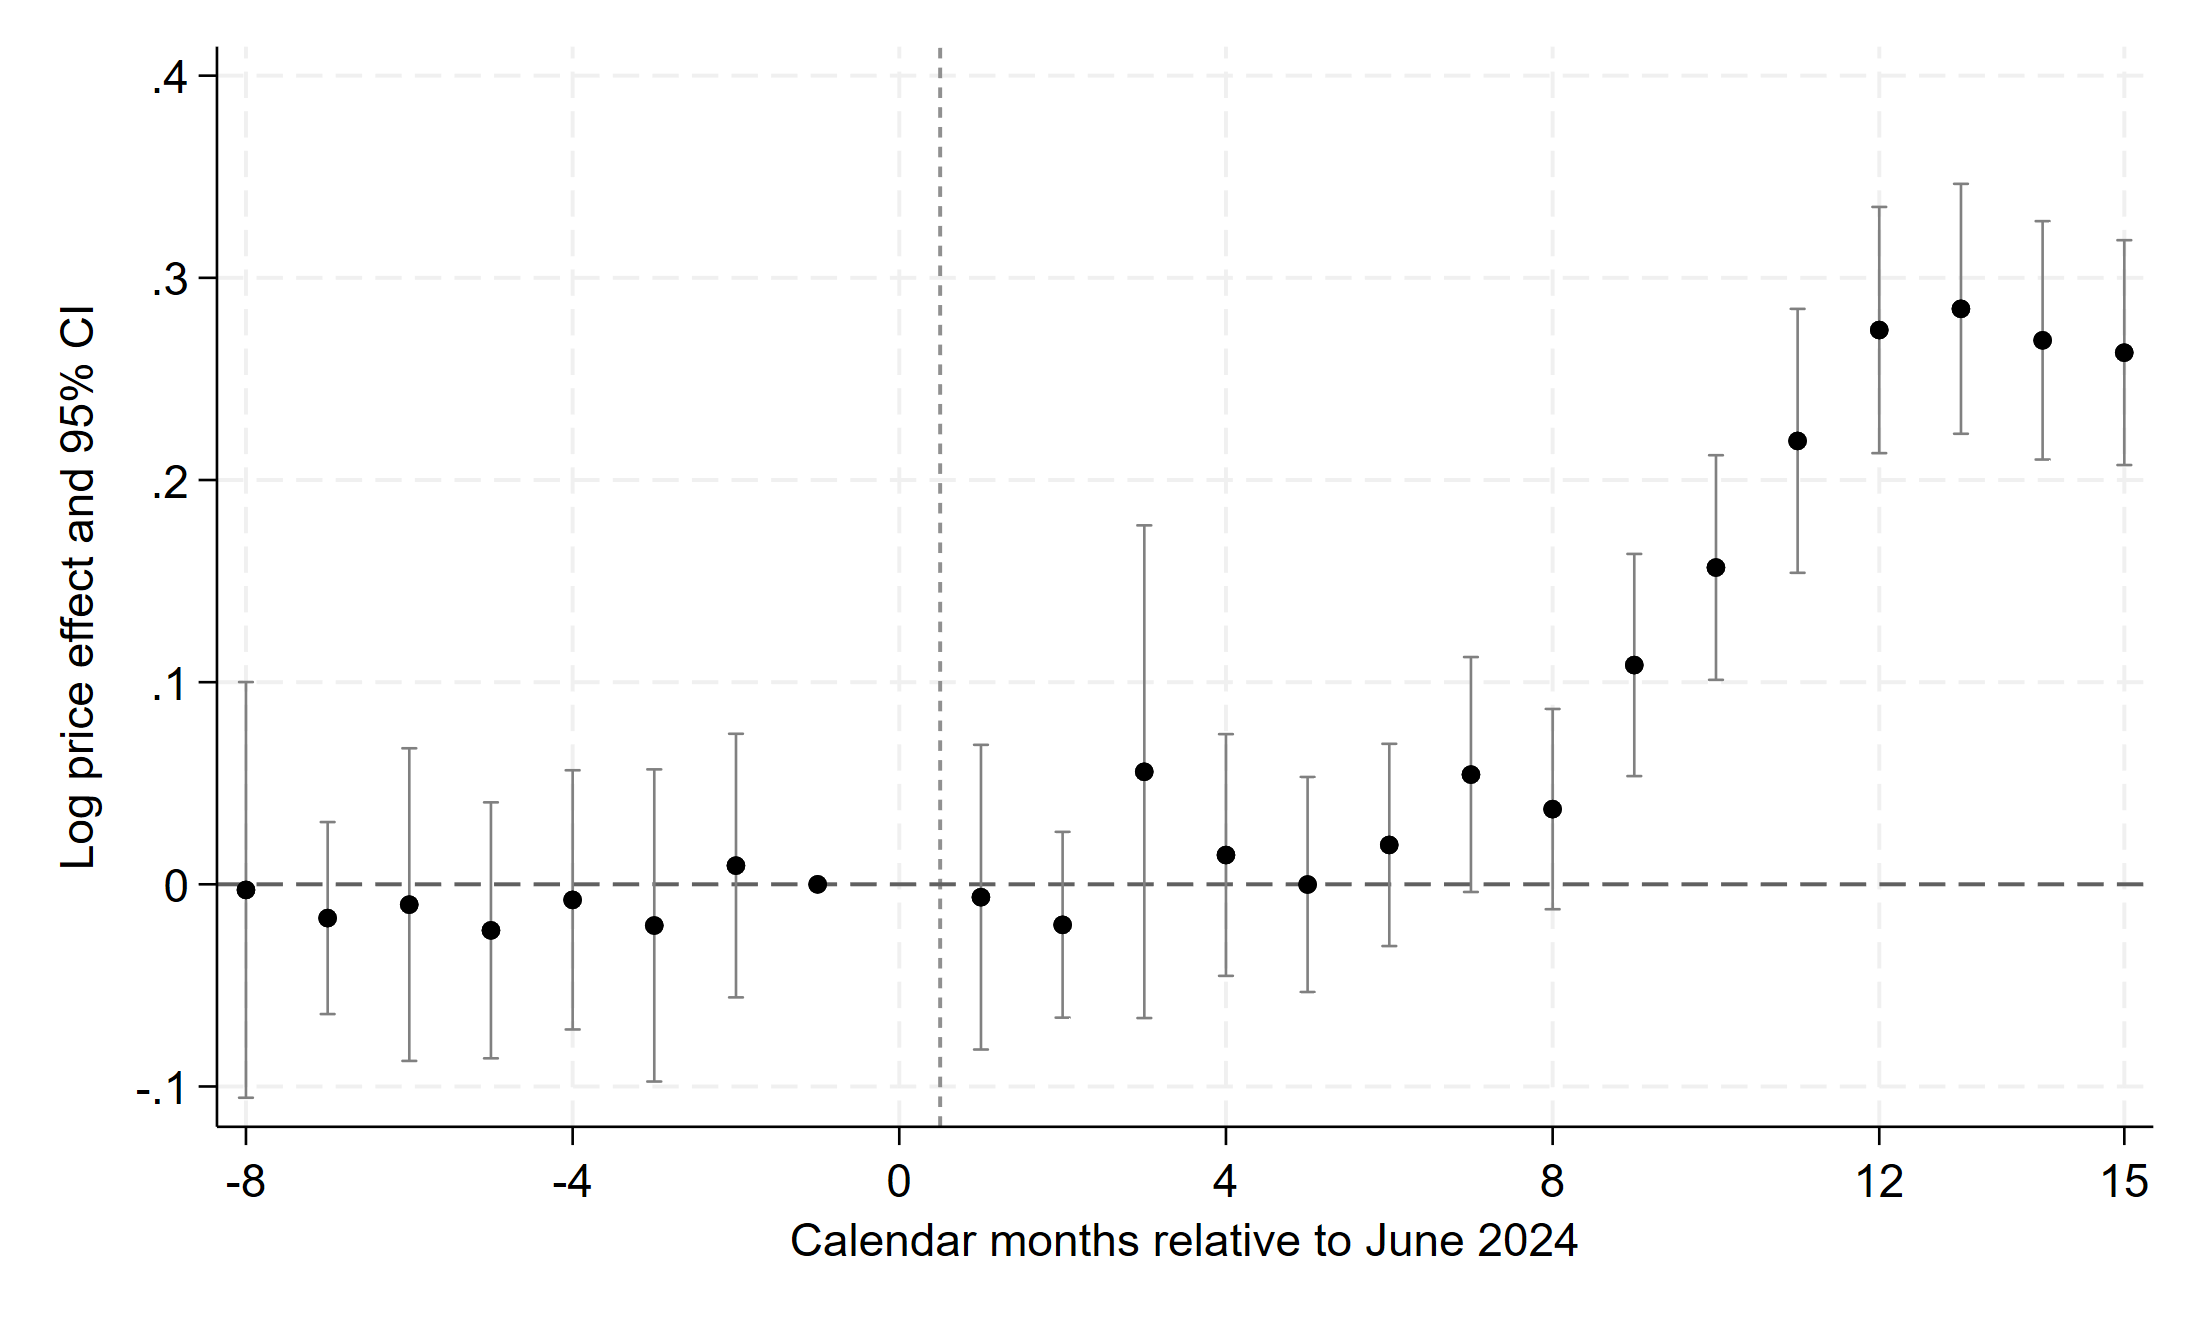
\includegraphics[width=\linewidth]{../outputs/figures/stata/micro_event_study.png}\end{minipage}\hfill
\begin{minipage}{0.49\linewidth}\centering\textbf{B. Official beef-minus-food CPI gap}\par\smallskip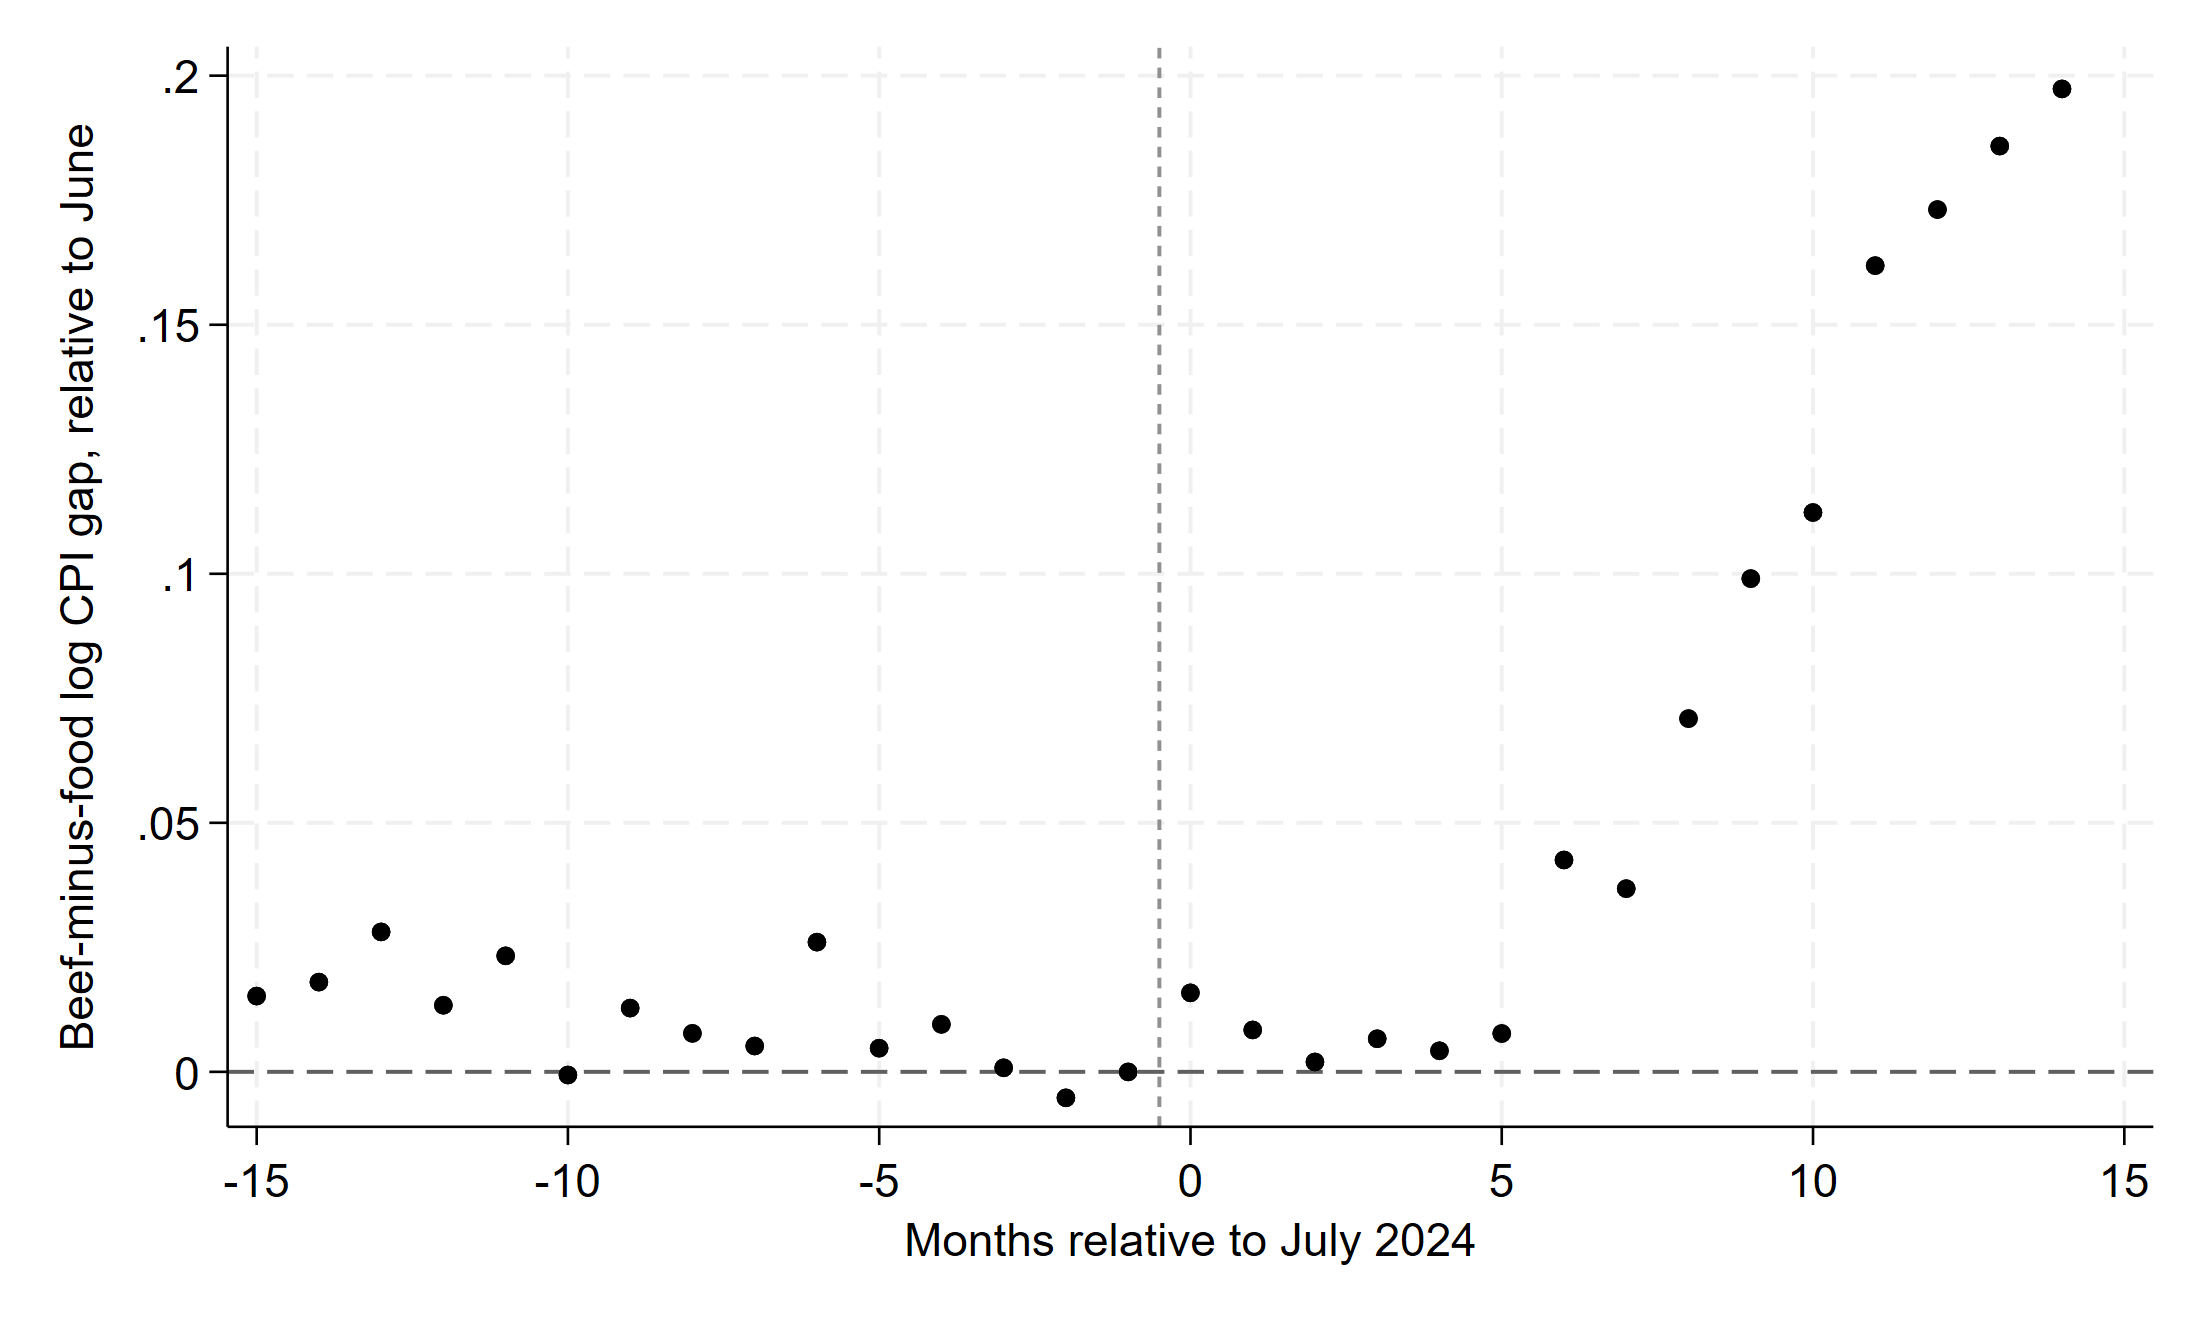
\includegraphics[width=\linewidth]{../outputs/figures/stata/aggregate_event_study.png}\end{minipage}
\figurenotes{dagligepriser.dk (Panel A); Statistics Denmark (Panel B).}{Panel A averages recorded changes, omits June 2024, uses May ($-1$) as reference, and preserves an empty event-month slot at zero. Its bars are product--store clustered intervals for the event-record regression only; they do not quantify national-policy uncertainty. Panel B shows monthly log CPI gaps relative to June 2024 without pointwise inference bars. July is $+1$ in Panel A and the first post month in Panel B. Both samples end in September 2025.}
\end{figure}

Appendix Figure~\ref{fig:b_country_sdid} displays the country beef HICP path underlying Table~\ref{tab:main}, column 3. The extra-EU bilateral-import diagnostic gives $-0.0801$ (pair-bootstrap standard error 0.0782). Bilateral pairs are not independent Danish policy episodes; the transformation and omission of intra-EU trade preclude interpreting this as a bound on total foreign substitution (Appendix Figure~\ref{fig:b_trade_sdid}).

The production analysis yields a main slaughter-weight ATT of $-0.0661$ (placebo standard error 0.0811), or a point estimate of about a 6.4 percent decline. Its 95 percent interval, $[-0.225,0.093]$, includes zero. With a longer, pre-treatment seasonally adjusted panel, the estimate is $-0.0055$. Slaughter counts show similarly uncertain responses. Direct estimation of log mean carcass weight on common country--months gives $-0.0184$ (placebo standard error 0.0258), with an interval spanning zero. Subtracting the separate weight and head-count ATTs would not estimate this outcome because their synthetic weights can differ. Appendix Table~\ref{tab:production} presents the slaughter estimates and June-omission check, and Table~\ref{tab:window_sensitivity} displays raw-log 15-, 24-, 36-, and 54-month estimates for every outcome. Production evidence does not establish the quantity contraction implied by the model, and the sensitivity across windows is relevant to interpreting the price results.

The negative sign of the main slaughter estimate is nevertheless consistent with the model's predicted contraction. Its economic magnitude depends in part on supply elasticity: a less elastic production technology limits quantity adjustment to a given change in expected net returns, while more elastic supply permits a larger response. In the model, the inverse supply elasticity $\eta$ enters together with demand elasticity and intertemporal adjustment costs. A small quantity response alongside rising prices could therefore be consistent with biological or capacity constraints, but the imprecise slaughter estimates do not establish that explanation.

The observed price--quantity combination does not by itself identify supply elasticity. The announcement shifts expected production costs, so the resulting equilibrium moves along demand as well as reflecting supply adjustment. Moreover, consumer prices and slaughterhouse output measure different stages of an internationally traded market. Taking the ratio of the slaughter ATT to the retail-price ATT would consequently not recover a supply elasticity. The evidence leaves both relatively rigid short-run supply and more responsive production compatible with the data; distinguishing them would require farm-level output and producer-price variation that isolates movements along supply.

The two-date model also disciplines magnitude. Even assigning the full 59.6 kg CO2e/kg lifecycle intensity to the future average output burden, the 2024-DKK rate of 125.93/tCO2e gives a wedge of about DKK 7.51/kg. For $\delta\leq1$, Corollary~\ref{cor:price_bound} limits the stationary two-date announcement price change to DKK 3.75/kg. The preferred CPI coefficient mapped to the screened grocery event-price mean corresponds to about DKK 9.79/kg. That numerical discrepancy would challenge a literal interpretation in which the entire retail contrast is produced by this mechanism with these primitives. The comparison crosses a retail CPI and an unvalidated grocery level anchor, uses lifecycle emissions broader than the tax base, and suppresses multiple production dates, trade, and retail margins. It therefore motivates the attribution sensitivity below rather than a rejection of anticipation.

\section{Conditional Environmental-Price Accounting}\label{sec:calibration}
The price estimates do not measure how much climate damage consumers internalize. I instead ask how a hypothesized policy-attributable price increment compares, in DKK/kg, with a selected environmental-damage benchmark. The exercise requires separate assumptions about causal attribution, persistence until 2030, additional price adjustment at implementation, and the taxable emissions base. I construct a literature benchmark, express it in beef-price units, and keep the announcement and implementation components distinct. This is conditional arithmetic, not a welfare estimate or an estimate of optimal retail pricing.

The benchmark gives equal weight to one selected estimate from each of ten studies \citep{cai2016,nordhaus2017,ricke2018,cailontzek2019,pindyck2019,hansel2020,vandenbremer2021,dietz2021,rennert2022,barrage2024}. This is a documented selection of the literature rather than an exhaustive systematic review. The studies differ in discounting, damage functions, risk, and the object valued. In particular, \citet{pindyck2019} estimates an average cost of avoiding catastrophic outcomes, which differs from the marginal SCC in the other studies. Excluding that estimate raises the pooled benchmark to USD 166.32/tCO2. Appendix Table~\ref{tab:scc} records the chosen estimates and the external comparisons.

Cai et al. (2016) reports both its initial SCC and monetary values for 2010. The inventory treats Pindyck's monetary base as 2017, an explicit valuation-date assumption; its exclusion sensitivity addresses this additional comparability issue. I inflate dollar values to 2024 US dollars and multiply values per ton of carbon by $12/44$ to obtain values per ton of CO2. The Cai--Lontzek input is the combined economic-and-climate-risk value of USD 124/tC for 2005 in their Table 9, with intertemporal elasticity 1.5 and risk aversion 10. The Barrage--Nordhaus 2030 value is log-interpolated between published 2025 and 2050 points. Only this value and Nordhaus's reported 2030 estimate refer directly to 2030; their two-study mean is USD 93.36/tCO2. The remaining values are held constant for the calibration. This is an imposed sensitivity assumption even when a study supplies a rising or stochastic future path. The ten-study mean should therefore be interpreted as a constant-value benchmark used in a 2030 exercise, rather than a pooled forecast for that year.

The equal-paper-weight point mean across ten studies is USD 160.39/tCO2. A sensitivity envelope is constructed in two explicit layers. Index papers by $j$. Let $\theta_j$ be paper $j$'s preferred harmonized SCC estimate and $[L_j,U_j]$ its reported positive central range. Let $1-2\alpha_j$ denote its reported coverage where available, or an assumed coverage for a parameter span. Let $\Phi$ denote the standard normal cumulative distribution function and define
\begin{equation*}
z_j=\Phi^{-1}(1-\alpha_j),\qquad
\sigma_j=\frac{\log U_j-\log L_j}{2z_j}.
\end{equation*}
Here $z_j$ is the corresponding standard-normal quantile and $\sigma_j$ is the calibrated log-scale standard deviation. For a selected paper with a usable range, the within-paper draw is
\begin{equation*}
X_j=\exp\!\left(\log\theta_j-\tfrac12\sigma_j^2+\sigma_j Z_j\right),
\qquad Z_j\sim N(0,1),
\end{equation*}
where $Z_j$ is an independent standard-normal variate, $X_j$ is the simulated SCC value, and $E[\cdot]$ denotes expectation. The $-\sigma_j^2/2$ adjustment ensures that $E[X_j]=\theta_j$, while the range's log width determines dispersion. Matching the arithmetic mean in this way generally means that $L_j$ and $U_j$ are not the simulated distribution's corresponding quantiles; the procedure matches their log width, not both endpoints. For papers without a positive range, $X_j=\theta_j$. The 66 percent model range in \citet{ricke2018} has $\alpha_j=0.17$ and therefore $z_j=\Phi^{-1}(0.83)$; the 5th--95th quantiles in \citet{rennert2022} have $\alpha_j=0.05$ and $z_j=\Phi^{-1}(0.95)$; and the ethical-parameter range in \citet{hansel2020} is assigned 95 percent coverage as an explicit sensitivity assumption, so $\alpha_j=0.025$ and $z_j=\Phi^{-1}(0.975)$.

In the second layer, each of 10,000 bootstrap replications samples ten papers with replacement from the ten-paper pool, makes an independent within-paper draw for every sampled paper, and records the arithmetic mean of those ten draws. Resampling papers describes sensitivity to the selected pool; the lognormal step adds dispersion calibrated to source ranges. Shared models and assumptions across studies mean that paper draws should not be interpreted as independent scientific replications. The 2.5th and 97.5th percentiles of the 10,000 replicated means are USD 79.50 and USD 366.63/tCO2. Because the inputs mix model, parameter, and distributional uncertainty rather than comparable sampling errors, this interval is a hierarchical sensitivity envelope, not a frequentist confidence interval for a common structural parameter.

Figure~\ref{fig:scc} shows each preferred estimate after mapping it into a hypothetical log beef-price equivalent net of the DKK 300/tCO2e marginal abatement incentive. This marginal rate is informative about emissions-reduction incentives; it is not the average burden on beef output. Filled points enter the pool. The hollow point is the external literature synthesis, whose inclusion could double count underlying studies \citep{moore2024}. The partial mortality SCC is reported separately in Appendix Table~\ref{tab:scc} \citep{carleton2022}. The triangle is the lower bound reported by \citet{bilal2026} and also remains external. The wide intervals reveal why retaining study-level variation materially changes the accounting comparison.

\begin{figure}[htbp]\centering
\caption{Selected SCC estimates and hypothetical beef-price equivalents}\label{fig:scc}
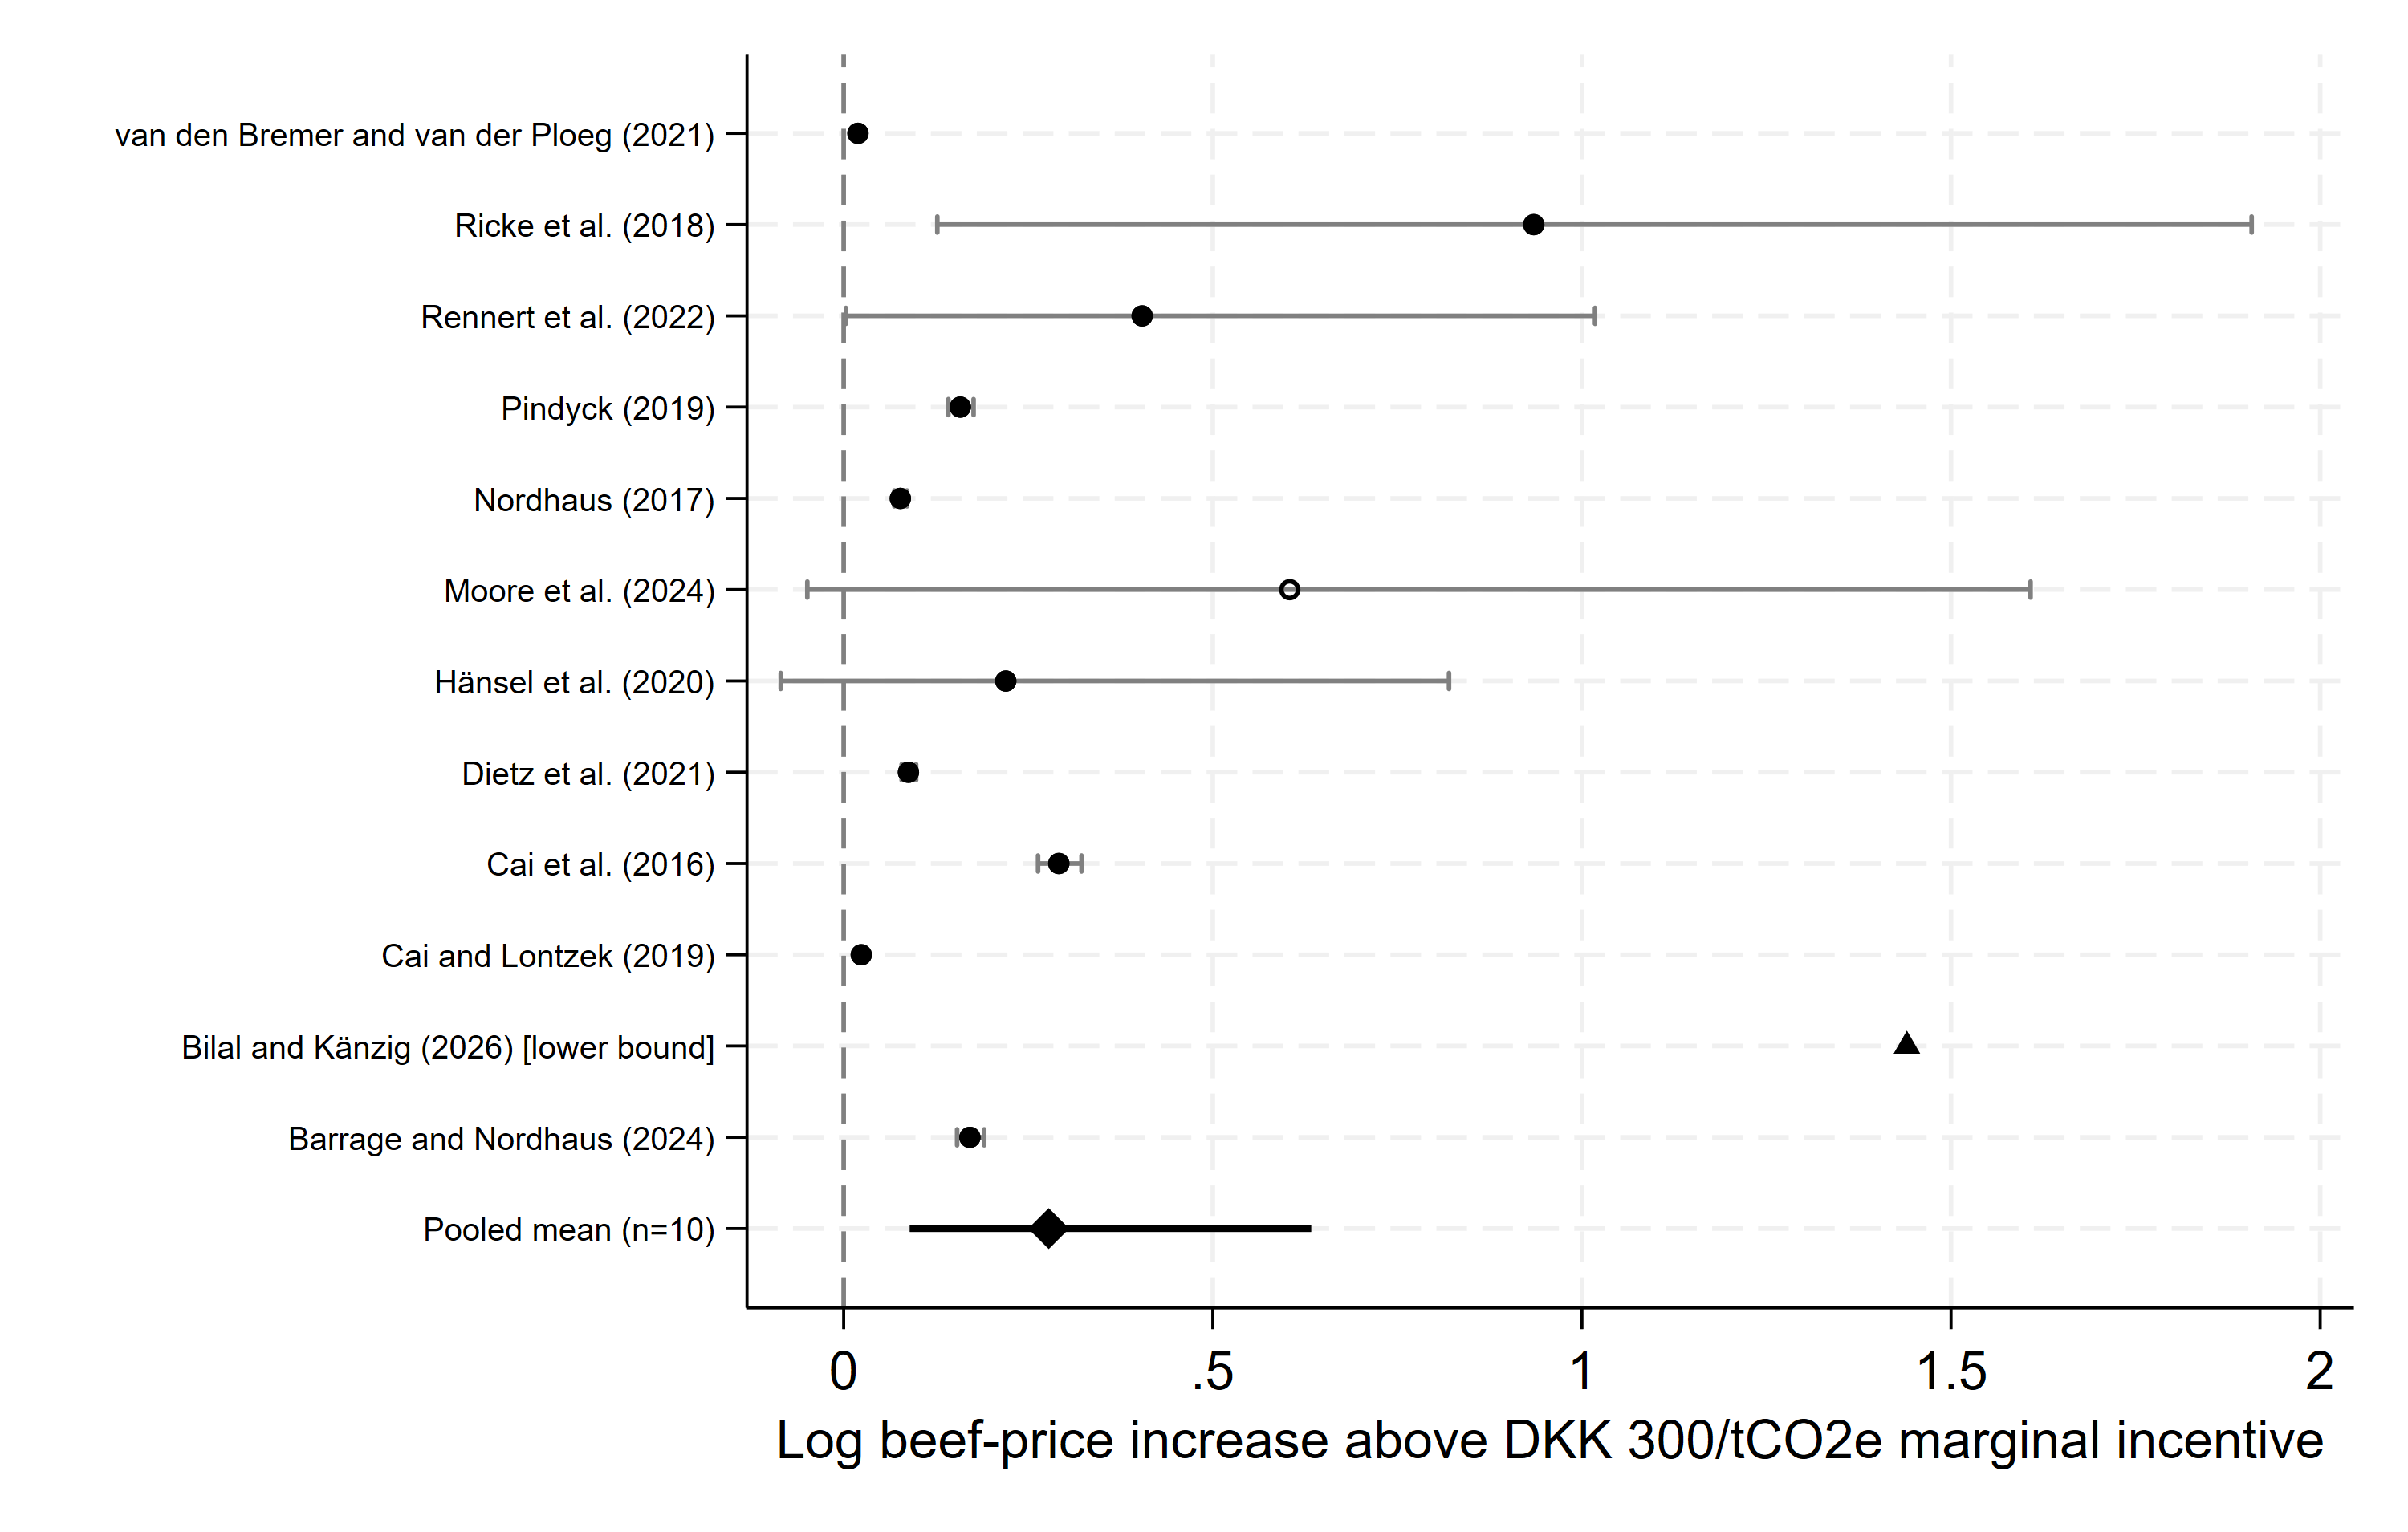
\includegraphics[width=0.98\linewidth]{../outputs/figures/stata/scc_meta_forest.png}
\figurenotes{The studies listed in Appendix Table~\ref{tab:scc}; \citet{oecd2025}.}{Each point maps a preferred SCC estimate into the log beef-price increase needed above the DKK 300/tCO2e marginal incentive, using a 59.6 kg CO2e/kg lifecycle benchmark, 6.8953 DKK/USD, and the scraped pre-announcement beef price. The quoted 2022-DKK statutory rate is converted to 2024 DKK using the annual net-price index. The lifecycle benchmark is broader than the farm-level emissions base subject to the Danish levy, so the mapping is an accounting sensitivity rather than a tax-base calculation. Bars show simulated 2.5th--97.5th percentile sensitivity intervals combining available SCC ranges with resampling of the grocery price benchmark. SCC values without a usable range are held fixed; their bars capture price resampling alone. The lower-bound triangle is conditional on the central price benchmark and has no simulated interval. Original source ranges remain in Appendix Table~\ref{tab:scc}. Filled circles enter the equal-paper-weight pool; hollow circles and the lower-bound triangle do not. The pooled diamond maps the mean SCC; its line combines hierarchical SCC and price-benchmark draws.}
\end{figure}

Let $\bar p=147.25$ be the provisional mean pre-announcement beef change-event price in DKK/kg, $r^{FX}=6.8953$ DKK/USD the exchange rate, and $\widetilde{\chi}=59.6$ kg CO2e/kg beef the lifecycle carbon-intensity benchmark. The benchmark follows the OECD's presentation of the beef-herd estimate from \citet{poore2018} \citep{oecd2025}. It includes lifecycle emissions beyond the farm-level emissions base to which the Danish levy applies. Equation~\eqref{eq:scc_gap} is therefore a deliberately broad accounting sensitivity and can overstate the price-equivalent wedge if $\widetilde{\chi}$ is interpreted as taxable emissions intensity. Neither the OECD presentation nor the accompanying source tables provide a sampling interval for this specific intensity benchmark. Their producer-level percentiles describe heterogeneity across production systems, rather than uncertainty in the mean used here. I therefore hold $\widetilde\chi$ fixed; the scenarios for $f$ below address the assumed taxable share, without assigning it a probability distribution.

The grocery level anchor is itself estimated from selected change-event months. I resample complete product--store histories and common circular blocks of two consecutive pre-announcement months, recomputing the observation-weighted mean in each replication. This preserves repeated observations within products and allows for shared monthly movements. The 412 observations cover 156 product--store pairs but only eight months. The resulting 2.5th--97.5th percentile range is DKK 131.04--165.40/kg. This range is only resampling sensitivity: it cannot correct the missing availability history, selective coverage, or package mismeasurement. One- and four-month blocks give similar ranges. I pair these draws independently with the SCC draws when constructing the mapped intervals in Figures~\ref{fig:scc} and~\ref{fig:policy}. At the individual-study level, the same lognormal range calibration is used where available, including the external synthesis; other SCC point estimates are held fixed. Thus these bars need not reproduce the original source ranges, which remain reported in the appendix.

For SCC value $c^{SCC}$ in USD/tCO2 and Danish rate $\tau$ in DKK/tCO2, define the additional log price required as
\begin{equation}\label{eq:scc_gap}
g(c^{SCC};\tau)=\log\left[\frac{\bar p+(c^{SCC}r^{FX}-\tau)\widetilde{\chi}/1000}{\bar p}\right].
\end{equation}
Here $c^{SCC}$ denotes the SCC input. The quoted statutory rates are DKK 120 and DKK 300 in 2022 prices. Annual Danish net-price indices imply a 2024/2022 factor of 1.04938; hence $\tau$ is evaluated at 125.93 and 314.81 in 2024 DKK. The former is the effective average output burden created by the 60 percent per-animal deduction; the latter is the 2030 marginal abatement incentive \citep{danishgovernment2024,danishtaxministry2024}. At the central calibration, $c^{SCC}=\bar c^{SCC}\equiv J^{-1}\sum_{j=1}^{J}E[X_j]$, where $J=10$ is the number of eligible papers. Because the within-paper draws are centered so that $E[X_j]=\theta_j$, $\bar c^{SCC}$ is the equal-paper-weight mean. In each bootstrap replication, $c^{SCC}$ is replaced by that replication's arithmetic mean, and the price benchmark is replaced by its paired resampled mean.

At the pooled mean, the hypothetical log-price equivalent is 0.334 under the average-burden benchmark, with a sensitivity range of 0.155--0.674. Under the marginal-incentive benchmark, it is 0.278, with a range of 0.089--0.633. Figure~\ref{fig:policy} places these accounting magnitudes alongside the official econometric estimates. The ATT intervals retain their econometric interpretation, while the accounting ranges combine SCC and provisional grocery-level sensitivity. Their overlap is not a formal test of the difference between the ATT and the calibrated equivalent. Across leave-one-study-out calculations, the SCC mean ranges from USD 111.56 to USD 172.36/tCO2, showing the influence of the highest estimate on the central benchmark.

\begin{figure}[htbp]\centering
\caption{Observed price contrasts and hypothetical SCC price equivalents}\label{fig:policy}
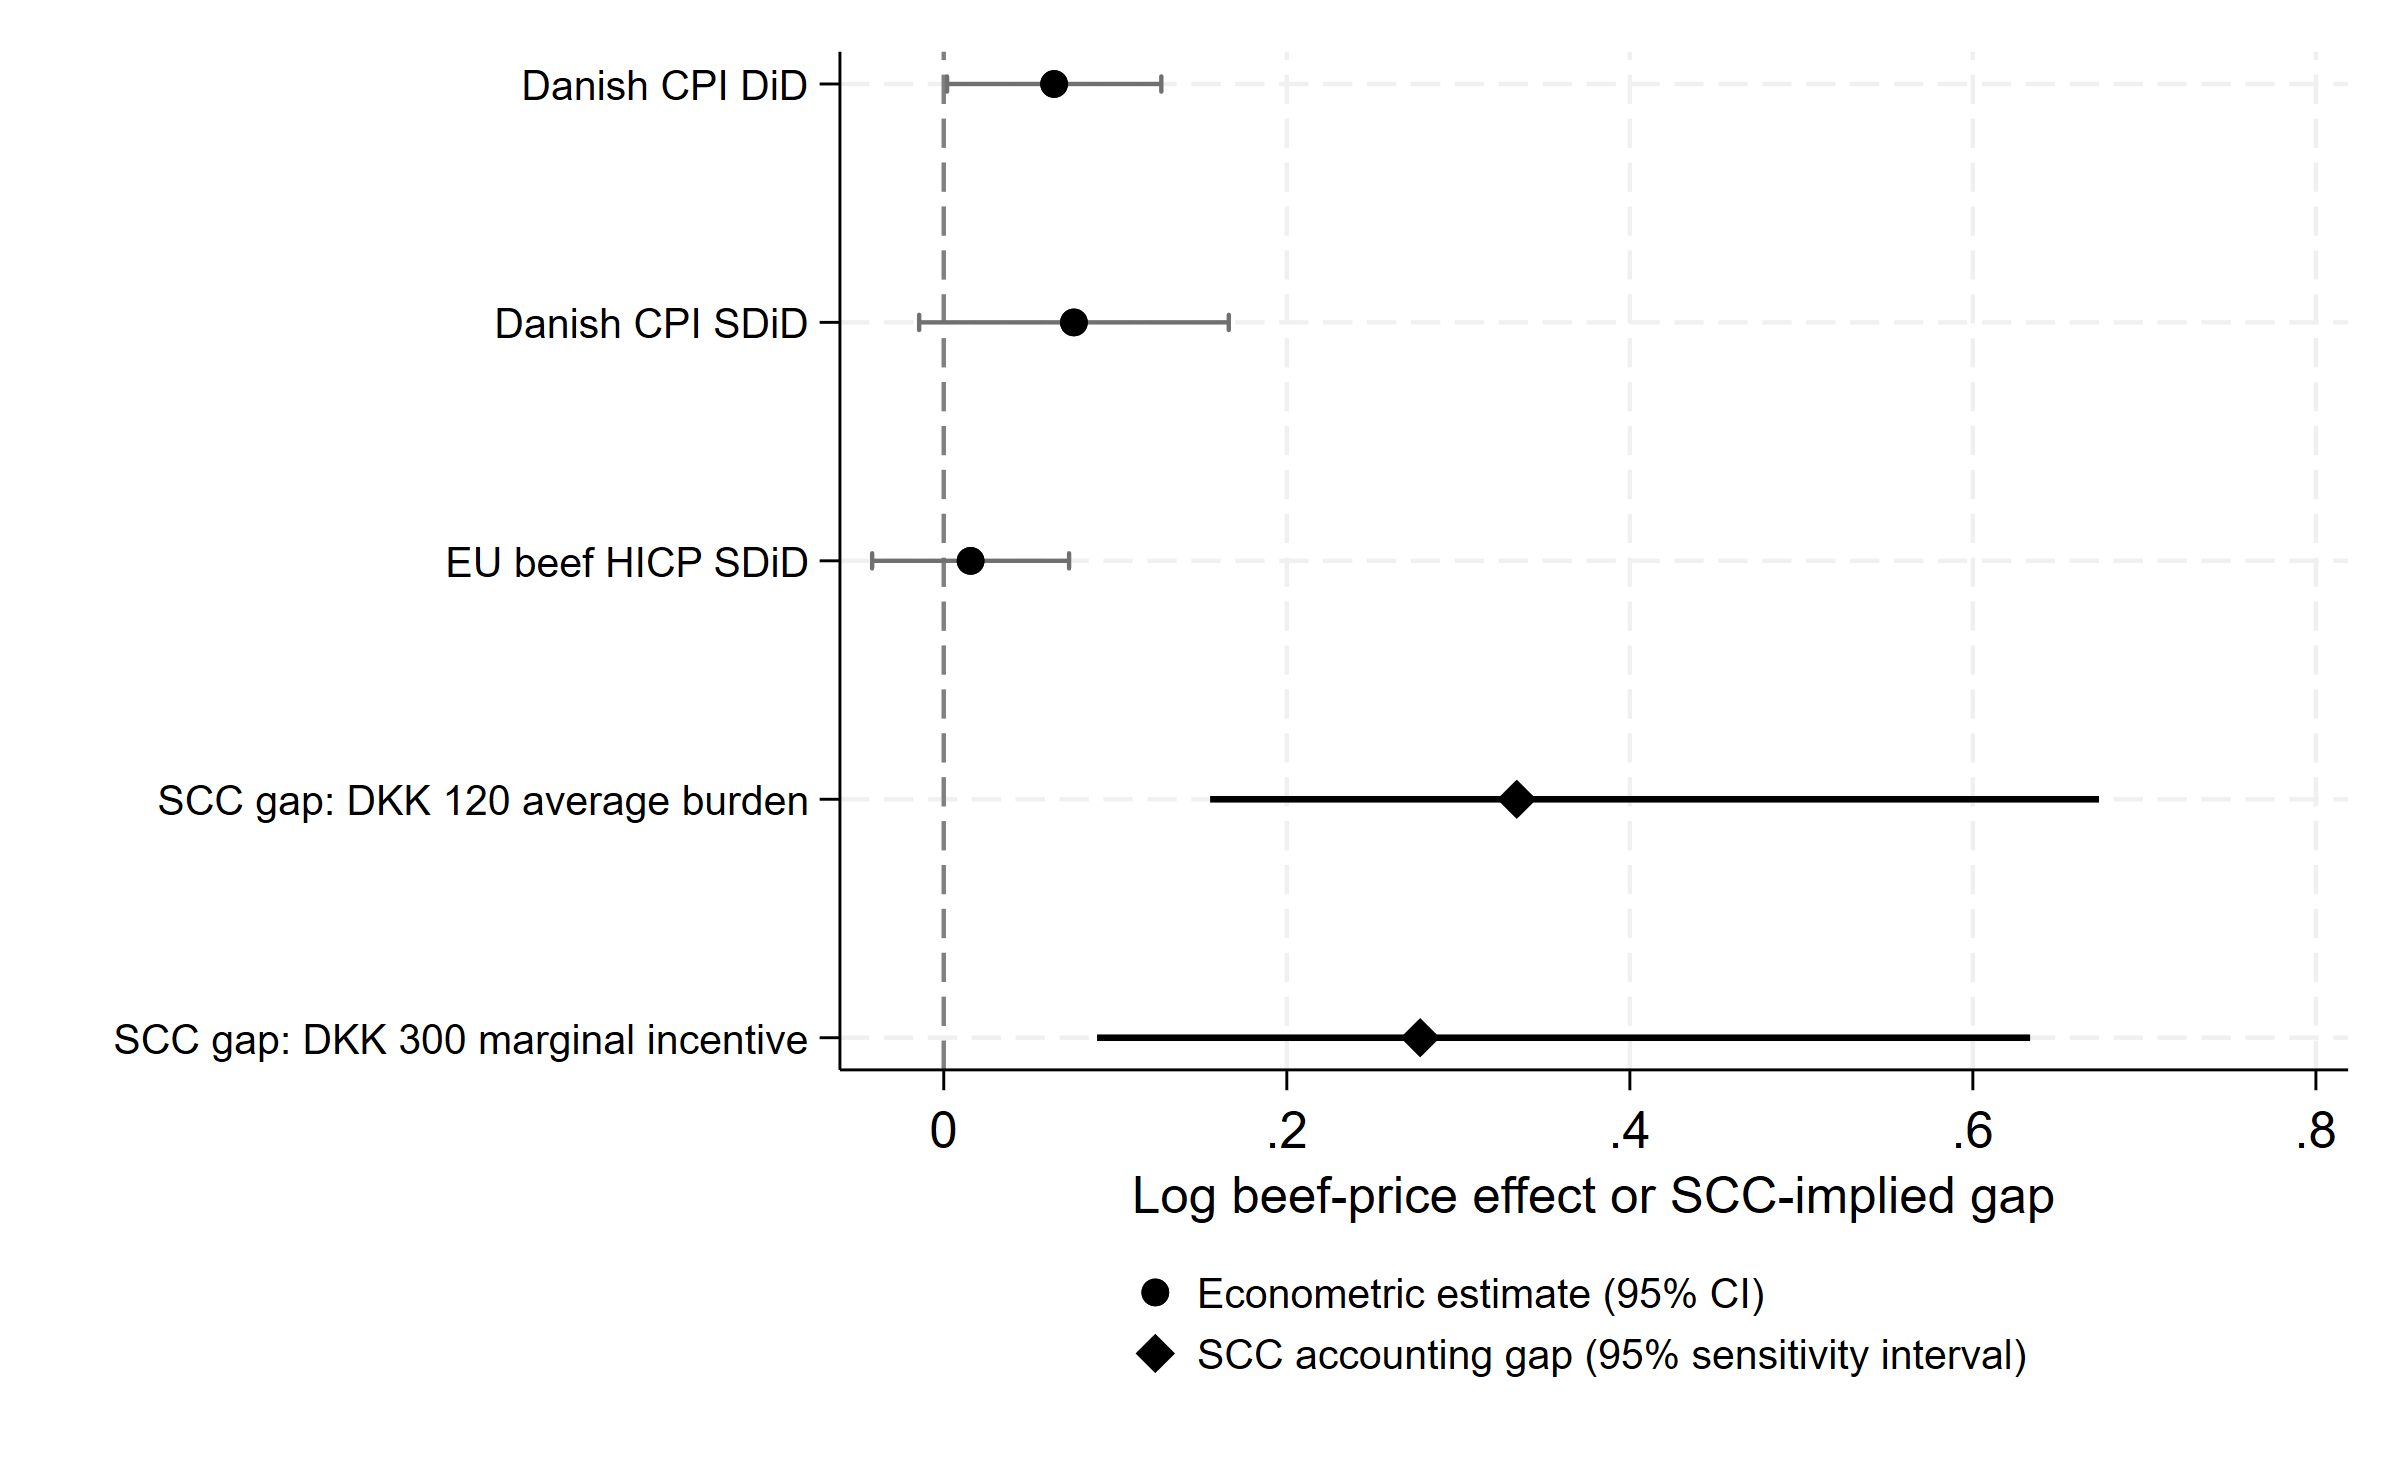
\includegraphics[width=0.92\linewidth]{../outputs/figures/stata/beef_policy_calibration.png}
\figurenotes{Statistics Denmark; dagligepriser.dk; the studies listed in Appendix Table~\ref{tab:scc}.}{Points show the three ATT estimates in Table~\ref{tab:main} and the SCC-implied log gaps under the DKK 120/tCO2e effective average output burden and DKK 300/tCO2e marginal abatement incentive. Quoted statutory rates are in 2022 DKK and are converted to 2024 DKK before calculation. Horizontal bars are 95 percent econometric intervals or the mapped 2.5th--97.5th percentile sensitivity interval combining hierarchical SCC draws and independent resampled grocery-price means. The ATT intervals do not depend on the level-price benchmark and retain their original standard errors. The 59.6 kg CO2e/kg lifecycle benchmark is broader than the levy tax base. These are accounting comparisons, not estimates of the taxable emissions base, tax incidence, or welfare.}
\end{figure}

To connect the calculation to the question posed at the start of this section, let $q\in[0,1]$ be the assumed share of the observed price contrast attributable to the cattle-policy episode, $a\in[0,1]$ the fraction of that attributed increment persisting until implementation, $f\in[0,1]$ the fraction of lifecycle emissions used as a taxable-intensity approximation, and $\lambda\in[0,1]$ additional implementation pass-through relative to the reference-animal average burden. The remaining hypothetical level difference in DKK/kg is
\begin{equation}\label{eq:persistence_gap}
R(q,a,f,\lambda)=\frac{\bar c^{SCC}r^{FX}\widetilde\chi}{1000}
-qa\bar p(e^{\widehat\beta}-1)
-\lambda\tau^{avg}_{2024}\frac{f\widetilde\chi}{1000},
\end{equation}
where $\widehat\beta=0.0644$ is the preferred official-price DiD estimate in column 1 of Table~\ref{tab:main} and $\tau^{avg}_{2024}=125.93$. The parameter $q$ is not estimated: the country-HICP comparison, 2025 timing, and nitrate-derogation change give reasons to consider values below one, including zero. The last term represents an \emph{additional} price increment after the announcement period. If a pass-through estimate instead measures total incidence including earlier adjustment, that total must replace the two price terms together. This distinction prevents counting the same adjustment twice. The marginal abatement rate is excluded from this output-price decomposition because the fixed deduction separates marginal emissions incentives from the average output burden.

The CPI estimate is a proportional contrast rather than a DKK/kg change. Applying it to $\bar p$ assumes that the same proportional movement applies to the selected grocery change-event level. At $q=1$, this maps the preferred estimate to DKK 9.79/kg, while the pooled lifecycle-damage benchmark is DKK 65.91/kg. Under full attribution and persistence with no additional implementation increase, the hypothetical difference is DKK 56.12/kg. With full additional pass-through and the broad assumption $f=1$, it falls to DKK 48.62/kg. At $q=0$ with the same full additional pass-through and taxable share, it is DKK 58.41/kg. Thus attribution is a separate substantive assumption, not absorbed into persistence.

Figure~\ref{fig:surfaces} sets $q=1$ to show the upper-attribution scenario, varies announcement persistence $a$ and additional implementation pass-through $\lambda$ over $[0,1]$ in four panels, and holds taxable share $f\in\{0.25,0.50,0.75,1\}$ by panel. Each surface is a plane: persistence subtracts the same assumed attributed increment at every pass-through value, while the slope with respect to pass-through becomes steeper as the taxable share rises. At $q=0$, persistence has no effect on the calculation. A narrow tax base limits the hypothetical additional price signal even when pass-through is complete. The panels describe conditional scenarios, not parameter forecasts.

The dashed surfaces combine uncertainty in the preferred price coefficient, the hierarchical SCC variation, and the resampled grocery price benchmark. For each of the 10,000 SCC draws, I independently draw a price coefficient centered on the preferred estimate, using its HAC standard error and a Student $t$ distribution with 28 degrees of freedom, matching the reference distribution used for Table~\ref{tab:main}. I also substitute a resampled price mean into equation~\eqref{eq:persistence_gap}, then report the 2.5th and 97.5th percentiles of the resulting gap at each parameter combination. Independence across these three draws is an explicit simulation assumption. In particular, covariance between the grocery benchmark and the official-price estimate is not estimated, although both may respond to common market shocks. Emissions intensity, the exchange rate, and the policy rate remain fixed. The resulting bounds are pointwise combined sensitivity intervals, conditional on these assumptions, rather than frequentist confidence bands. At $a=0$, both coefficient and price-benchmark uncertainty drop out, while SCC variation remains.

Even at $q=a=f=\lambda=1$, the combined 2.5th--97.5th percentile sensitivity range for the hypothetical difference is DKK 12.41--133.36/kg. Its width reflects variation in selected damage estimates, the price coefficient, and the provisional level anchor; it is not a sampling interval for a common SCC. Alternative month-block lengths give similar bounds. The smallest central difference in the stated scenario cube is DKK 48.62/kg, so none of these combinations closes the arithmetic difference at the selected damage benchmark. Under full attribution, persistence and additional pass-through, the two assumed price increments sum to about 26 percent of that benchmark. With no additional implementation response, the mapped CPI increment is about 15 percent. At full attribution and pass-through, equality would require an SCC of about USD 42.09/tCO2; a smaller taxable share or weaker attribution lowers that threshold. These calculations do not imply that observed prices internalize environmental damages.

\begin{figure}[p]\centering
\caption{Hypothetical environmental-price difference at implementation, full attribution}\label{fig:surfaces}
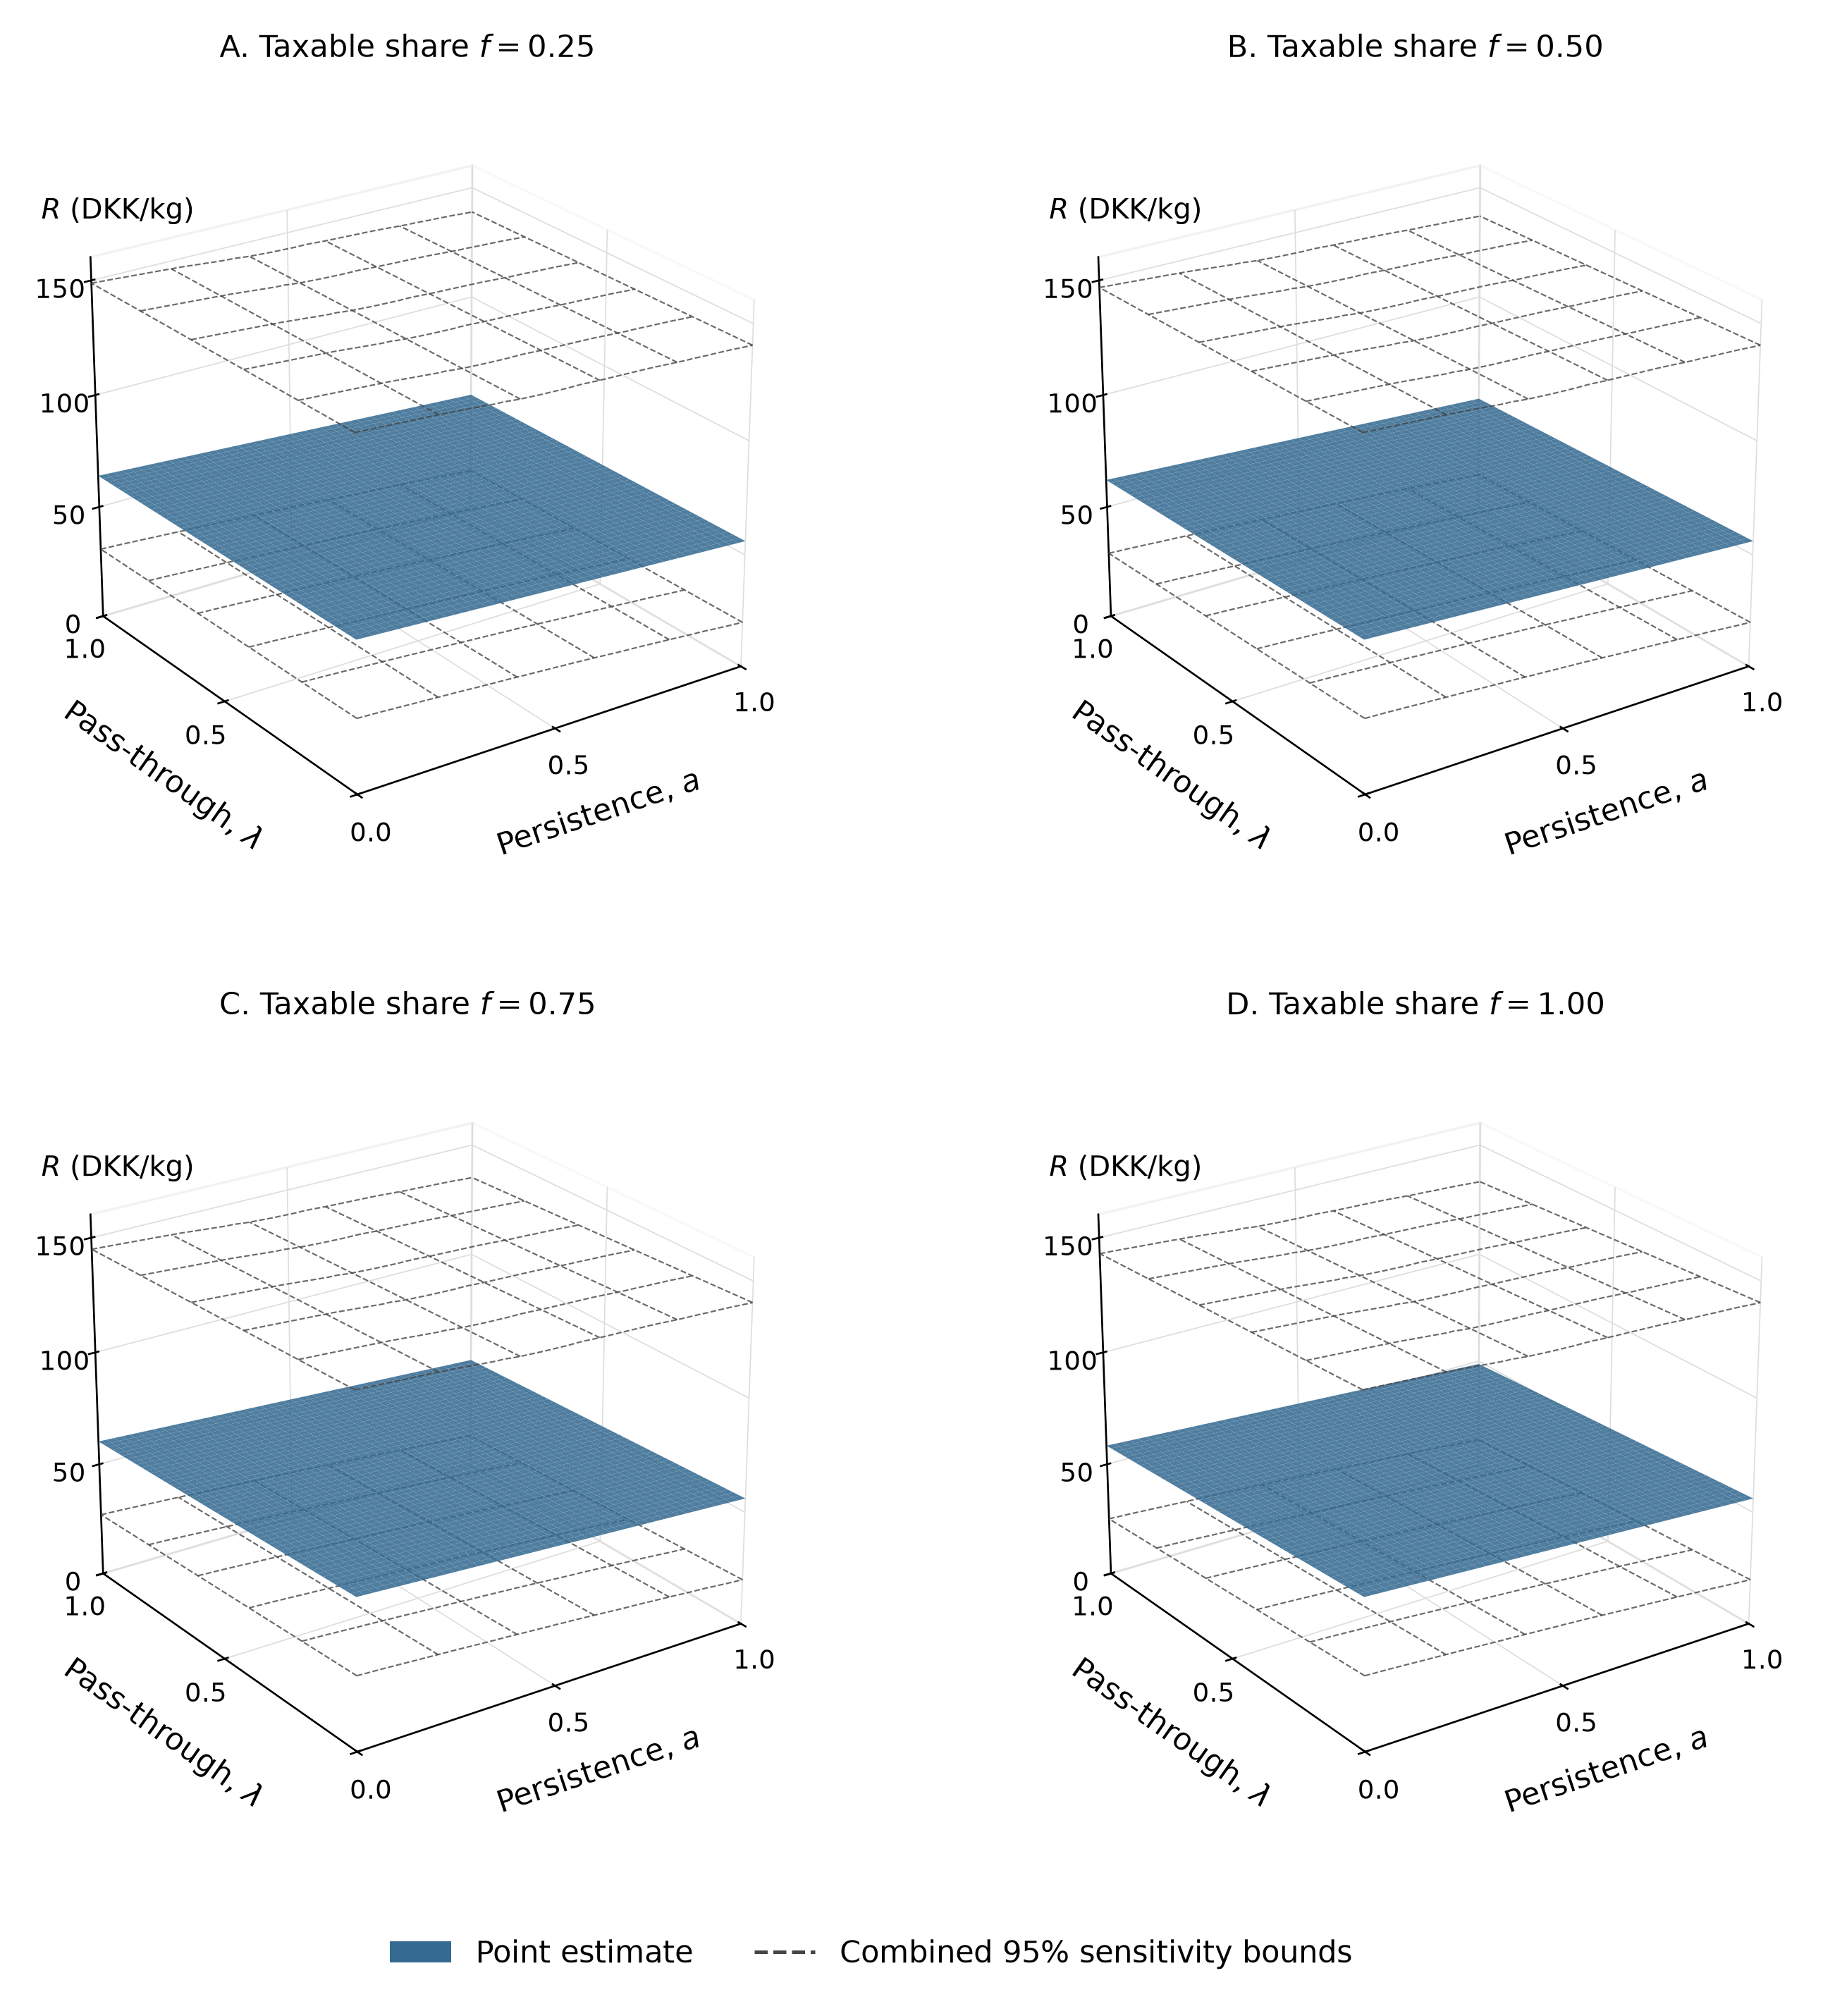
\includegraphics[width=0.95\linewidth]{../outputs/figures/python/calibration_surfaces.png}
\figurenotes{Statistics Denmark; dagligepriser.dk; the SCC studies in Appendix Table~\ref{tab:scc}.}{The vertical axis gives $R$ in DKK/kg from equation~\eqref{eq:persistence_gap}, setting attribution share $q=1$ and using the preferred official-price DiD in Table~\ref{tab:main}, column 1. Panels vary persistence $a$ and additional pass-through $\lambda$, holding taxable share $f$ at the indicated value. Solid surfaces show point estimates. Dashed meshes show pointwise 2.5th--97.5th percentile bounds combining hierarchical SCC draws, resampled grocery-price means, and coefficient draws using the HAC standard error and Student $t(28)$ distribution. Independence across these sources is assumed. These are conditional sensitivity intervals, not sampling confidence bands for a common SCC or simultaneous confidence bands. Intensity, exchange rate, and tax rate stay fixed; the sources provide no sampling interval for the specific intensity benchmark. All panels share the same vertical scale.}
\end{figure}

The exercise illustrates how strongly the arithmetic depends on attribution, the selected SCC studies, emissions intensity, the retail level anchor, and a possible later price response. Lifecycle CO2e combines gases with different timing and damage profiles; the pre-announcement grocery mean spans several months rather than a single 2024 valuation date; and Danish production is linked to international markets. The calculation uses a common real-price approximation and a one-for-one CO2e valuation convention. It cannot establish that any observed price movement represents internalized climate damages or identify the optimal Danish tax.

\section{Discussion of the Results}\label{sec:discussion}
The analysis asks whether environmental-policy announcements can influence markets before implementation. The model provides one mechanism: current production plans adjust when credible news changes expected future costs. The preferred Danish beef-versus-food CPI contrast is positive, but it appears mainly in 2025 and is sensitive to the HAC bandwidth. Denmark's beef HICP rises much less relative to the same product in other EU countries. These comparisons leave the size, timing, and cause of a Danish-specific announcement response uncertain. The grocery change-event regression cannot resolve that uncertainty.

The production results help assess this interpretation. A contraction in Danish slaughter output relative to other EU countries would support one observable implication of the planned-supply model. The main estimate has that sign, but its uncertainty is substantial and the longer-pre-period estimate is close to zero. The evidence therefore does not confirm the joint prediction of higher prices and lower output. It also does not exclude that prediction. Slaughterhouse activity measures only one stage of production, while herd composition, live-animal trade, emissions intensity, and procurement arrangements may adjust on different horizons.

The international checks serve distinct purposes. Comparing beef-and-veal consumer-price indices across countries addresses reliance on other foods as controls. This comparison gives a smaller, statistically insignificant point estimate. Differences in national beef-market developments and possible spillovers into donor countries remain relevant to identification, so the evidence warrants caution about the magnitude of the announcement response. The extra-EU import analysis examines one possible offset to domestic supply changes. Its interval includes economically relevant increases and decreases. Moreover, it excludes intra-EU trade, so it cannot establish the absence of an import response or verify the absence of spillovers into donor countries. Taken together, these exercises broaden the evidence while leaving the core identifying restrictions conditional.

The nitrate-derogation change is a particularly important limitation. It was announced before the livestock-tax agreement and took effect near the beginning of the post-period. Both measures can change expected cattle-production costs. Neither national food comparisons nor cross-country cattle comparisons distinguish their effects with these aggregate data. The broader Green Tripartite package also includes land-use and other agricultural measures. Interpreting the estimates as the isolated causal effect of a future emissions tax would require additional variation in exposure to these measures.

The conditional accounting exercise translates selected SCC values into hypothetical beef-price units. At the pooled literature benchmark, even assuming full causal attribution and persistence of the preferred CPI contrast and full additional implementation pass-through leaves a substantial arithmetic difference. Zero attribution yields a larger difference. Neither case measures a welfare gap: retail prices need not equal marginal external damages, the lifecycle benchmark exceeds the tax base, and the studies do not provide a common 2030 SCC distribution. These features preclude using the exercise to infer a uniquely appropriate Danish tax rate.

The model shows why credibility can matter before collection begins and gives an upper bound under its two-date assumptions. The observed CPI-to-level mapping exceeds that bound even under a generous lifecycle-intensity mapping of the average output burden. This comparison does not falsify the mechanism because it crosses different market levels and suppresses trade and multiple adjustment dates. It does make a full-attribution interpretation demanding. Establishing a welfare effect empirically would require quantities and emissions as well as prices, farm-level policy exposure, and attention to distributional incidence and trade leakage.

Several measurement issues remain relevant. The grocery history selectively records changes and lacks historical availability; its package normalization is partly heuristic. Official CPI avoids that event-selection problem but has one treated series and a limited donor set. Livestock products, including poultry and eggs, are excluded from the food donor pool, yet substitution and exposure to other parts of the agreement can still affect remaining foods. The country HICP check changes the control group while retaining the Danish statistical provider. Finally, surveillance detected the affected dairy herd in September 2025, before the officially dated October BVD outbreak interval \citep{dvt2025,dvfaBVD}. Ending the sample in September reduces exposure to the later outbreak without ensuring that cattle markets were unaffected in the final month.

\clearpage
\section{Conclusion}\label{sec:conclusion}
This paper examines beef markets during a policy transition that included news of a future livestock-emissions charge. A model with costly changes in production plans predicts that a credible future output burden can reduce current planned production and raise current prices, while a fixed-stock slaughter-timing mechanism can reverse the price sign. The preferred Danish beef-versus-food CPI contrast is positive, concentrated in 2025, and sensitive to the serial-correlation adjustment. The same-product EU-country HICP estimate is smaller and uncertain. The grocery change-event history does not supply an independent monthly-price check, and the slaughter estimates do not establish a corresponding contraction.

Announcements belong in the evaluation window, but the available comparisons cannot attribute the observed price path to the emissions tax alone. The end of Denmark's cattle nitrate derogation overlaps the post-period, European beef-price pressure was present in 2025, and production estimates depend on temporal support and adjustment. The SCC exercise reports hypothetical price equivalents conditional on attribution and tax-base assumptions, without measuring internalized damages. Archived posted-price spells, farm-level measures of herd adjustment and emissions, total trade flows, and variation in exposure to the nitrate and tax measures would help distinguish these channels as implementation approaches.

\clearpage
\bibliographystyle{apalike}
\bibliography{references}

\clearpage
\appendix
\renewcommand{\thetable}{A\arabic{table}}\renewcommand{\thefigure}{A\arabic{figure}}\renewcommand{\theequation}{A\arabic{equation}}\setcounter{table}{0}\setcounter{figure}{0}\setcounter{equation}{0}
\section{Theory Appendix}\label{app:theory}

\subsection{Proof of Proposition~\ref{prop:anticipation}}
The interior first-order conditions for \eqref{eq:potential} are
\begin{align}
G_0'(Q_0)+\delta\kappa(Q_T-Q_0)&=0,\label{eq:foc0}\\
G_T'(Q_T)-\omega-\kappa(Q_T-Q_0)&=0.\label{eq:foct}
\end{align}
Define $h_0\equiv-G_0''(Q_0)>0$, $h_T\equiv-G_T''(Q_T)>0$, and
\begin{equation*}
\Delta\equiv(h_0+\delta\kappa)(h_T+\kappa)-\delta\kappa^2
=h_0h_T+h_0\kappa+\delta\kappa h_T>0.
\end{equation*}
Implicit differentiation of \eqref{eq:foc0}--\eqref{eq:foct} gives
\begin{equation*}
\begin{bmatrix}h_0+\delta\kappa&-\delta\kappa\\-\kappa&h_T+\kappa\end{bmatrix}
\begin{bmatrix}\partial Q_0/\partial\omega\\\partial Q_T/\partial\omega\end{bmatrix}
=\begin{bmatrix}0\\-1\end{bmatrix}.
\end{equation*}
Cramer's rule therefore yields
\begin{equation}\label{eq:general_cs}
\frac{\partial Q_0}{\partial\omega}=-\frac{\delta\kappa}{\Delta}<0,
\qquad
\frac{\partial Q_T}{\partial\omega}=-\frac{h_0+\delta\kappa}{\Delta}<0.
\end{equation}
Since $P_0'(Q_0)<0$, $\partial P_0/\partial\omega=P_0'(Q_0)\partial Q_0/\partial\omega>0$. The first expression in \eqref{eq:general_cs} is zero when $\kappa=0$ or $\delta=0$; when $\pi=0$, $\omega=\pi\tau\chi=0$ and there is no policy-induced change. This proves the proposition.

\subsection{Derivation of Corollary~\ref{cor:microfoundation}}
For $\varepsilon\neq1$, the marginal utility of beef in \eqref{eq:utility} is $Aq^{-1/\varepsilon}$; the logarithmic case gives the same expression at $\varepsilon=1$. Because the numeraire's marginal utility and price both equal one, the household's interior first-order condition is $p=Aq^{-1/\varepsilon}$, which proves \eqref{eq:isoelastic_demand}. Its elasticity is $-(dQ/dP)(P/Q)=\varepsilon$.

With capital fixed, the production constraint \eqref{eq:cobb_douglas} requires $X=(Q/(BK^{1-\alpha}))^{1/\alpha}$. Multiplication by the input price $v$ gives \eqref{eq:micro_cost}. Differentiation yields
\begin{equation*}
C'(Q)=\frac{v}{\alpha}(BK^{1-\alpha})^{-1/\alpha}Q^{1/\alpha-1}
=mQ^{\eta},
\qquad \eta=\frac{1-\alpha}{\alpha}>0.
\end{equation*}
Equating inverse demand and marginal cost at a static competitive equilibrium gives \eqref{eq:baseline_equilibrium}. At that equilibrium,
\begin{equation}\label{eq:micro_curvature}
h\equiv-G''(Q^*)=-P'(Q^*)+C''(Q^*)
=\frac{P^*}{Q^*}\left(\frac{1}{\varepsilon}+\eta\right)
=\frac{P^*}{Q^*}s.
\end{equation}
Stationarity and $\omega=0$ imply $Q_0=Q_T=Q^*$, so $h_0=h_T=h$ in \eqref{eq:general_cs}. Since $\rho=\kappa Q^*/P^*$, substituting \eqref{eq:micro_curvature} into \eqref{eq:general_cs}, multiplying quantity derivatives by $P^*/Q^*$, and using $\partial\log P/\partial\log Q=-1/\varepsilon$ gives \eqref{eq:micro_q0}--\eqref{eq:micro_price}. These are derivatives evaluated at the nonlinear model's stationary equilibrium, so no linear demand or marginal-cost schedule is assumed.

Let
\begin{equation*}
R(\delta,\rho)\equiv
\frac{\delta\rho}{\varepsilon s[s+\rho(1+\delta)]}
\end{equation*}
denote the coefficient in \eqref{eq:micro_price}. Direct differentiation gives
\begin{equation*}
\frac{\partial R}{\partial\delta}
=\frac{\rho(s+\rho)}{\varepsilon s[s+\rho(1+\delta)]^2}>0,
\qquad
\frac{\partial R}{\partial\rho}
=\frac{\delta}{\varepsilon[s+\rho(1+\delta)]^2}>0.
\end{equation*}
Thus proximity and adjustment curvature strengthen local announcement incidence. The factors $\pi$, $\tau$, and $\chi$ enter through $\widehat{\omega}=\pi\tau\chi/P^*$.

\subsection{Proof of Corollary~\ref{cor:price_bound}}
Write $x=G'(Q_0)$ and $y=G'(Q_T)$ under stationary primitives. The first-order conditions of \eqref{eq:potential} imply $x=\delta\kappa(Q_0-Q_T)$ and $y=\omega-\kappa(Q_0-Q_T)$, so $x+\delta y=\delta\omega$. If $Q_T\geq Q_0$, then $x\leq0$ and $y\geq\omega>0$, while strict decrease of $G'$ implies $y\leq x$, a contradiction. Thus $Q_T<Q_0$, $y>x>0$, and $x\leq\delta\omega/(1+\delta)$. Since $G'(Q^*)=0$, $Q_0<Q^*$. Weakly increasing marginal cost then gives
\begin{equation*}
P(Q_0)-P(Q^*)=x+C'(Q_0)-C'(Q^*)\leq x\leq\frac{\delta}{1+\delta}\omega.
\end{equation*}
The proof uses the output wedge and price at the same market stage. Retail margins and imported supply are outside its assumptions.

\subsection{Multi-period anticipation}
Consider dates $t=0,\ldots,N$ and implementation at $T\leq N$. Let $\mathbf{1}\{\cdot\}$ denote the indicator function. The multi-period potential is
\begin{equation}\label{eq:multi}
\sum_{t=0}^N\beta^t\left[G_t(Q_t)-\omega\mathbf{1}\{t\geq T\}Q_t\right]
-\sum_{t=1}^N\beta^t\frac{\kappa}{2}(Q_t-Q_{t-1})^2.
\end{equation}
Let $\mathcal H$ be its Hessian in $Q=(Q_0,\ldots,Q_N)'$ and define $\mathcal M\equiv-\mathcal H$. The restrictions $G_t''<0$, together with the nonnegative quadratic adjustment terms, make $\mathcal M$ positive definite. Its diagonal entries are positive, its only off-diagonal entries are non-positive adjacent adjustment terms, and for $\kappa>0$ it is irreducible. Hence $\mathcal M$ is a nonsingular tridiagonal M-matrix and $\mathcal M^{-1}$ is elementwise strictly positive. Differentiating the first-order conditions with respect to $\omega$ gives
\begin{equation*}
\mathcal M\frac{\partial Q}{\partial\omega}=-b,
\qquad b_t=\beta^t\mathbf{1}\{t\geq T\}\geq0.
\end{equation*}
Therefore $\partial Q/\partial\omega=-\mathcal M^{-1}b<0$ at every date. A credible future wedge thus propagates backward through the production plan.

Under the stationary microfoundations in \eqref{eq:utility}--\eqref{eq:micro_cost}, evaluate the local response at the zero-wedge equilibrium $Q_t=Q^*$. For interior pre-implementation dates $1\leq t\leq T-1$, differentiating the first-order conditions gives the homogeneous recurrence
\begin{equation*}
\kappa \psi_{t-1}-[h+\kappa(1+\beta)]\psi_t+\beta\kappa \psi_{t+1}=0,
\end{equation*}
where $\psi_t\equiv\partial Q_t/\partial\omega$ and $h=(P^*/Q^*)s$ is given by \eqref{eq:micro_curvature}. Writing the stable component as $\psi_t\propto r^{T-t}$ gives the polynomial $\kappa r^2-\mathcal B r+\beta\kappa=0$, where $\mathcal B=h+\kappa(1+\beta)$. This polynomial has roots $0<r_-<1<r_+$. Selecting the smaller root is exact for a semi-infinite preperiod under boundedness as $T-t\rightarrow\infty$ and gives an interior approximation for a long finite preperiod:
\begin{equation}\label{eq:root}
r_-=\frac{\mathcal B-\sqrt{\mathcal B^2-4\beta\kappa^2}}{2\kappa}\in(0,1),
\qquad \mathcal B\equiv h+\kappa(1+\beta).
\end{equation}
Thus the absolute magnitude of the negative stable component, which is proportional to $r_-^{T-t}$, declines geometrically with distance from implementation. On an arbitrary finite horizon, the exact path combines both characteristic roots, with coefficients fixed by the initial and terminal boundary conditions; equation~\eqref{eq:root} is not an exact global finite-horizon solution. The M-matrix sign result above remains exact. The geometric characterization is the multi-period counterpart to the role of $\delta=\beta^T$ in the two-date model.

\subsection{Welfare and the Pigouvian benchmark}
Assume tax revenue is rebated lump-sum, tax administration is costless, private and social discount factors coincide, adjustment costs are real resource costs, and emissions intensity $\chi$ is fixed so that output is the only abatement margin. With emissions $E_t=\chi Q_t$, social welfare in the two-date model is
\begin{equation}\label{eq:welfare}
W=G_0(Q_0)-D_0(\chi Q_0)+\delta\left[G_T(Q_T)-D_T(\chi Q_T)-\frac{\kappa}{2}(Q_T-Q_0)^2\right].
\end{equation}
At a given date, equating the private output wedge $\chi\tau_t$ to marginal environmental damage per unit of output $\chi D_t'(E_t)$ gives $\tau_t^P=D_t'(E_t)=MD_t^e$, proving \eqref{eq:pigou}. The paper's SCC comparison additionally imposes the one-for-one CO2e valuation convention stated in the main text.

Along the private equilibrium defined by \eqref{eq:foc0}--\eqref{eq:foct}, differentiation of \eqref{eq:welfare} and substitution of the first-order conditions yield
\begin{equation}\label{eq:welfare_derivative}
\frac{dW}{d\omega}
=-\chi D_0'(E_0)\frac{\partial Q_0}{\partial\omega}
+\delta[\omega-\chi D_T'(E_T)]\frac{\partial Q_T}{\partial\omega}.
\end{equation}
Both quantity derivatives are negative by Proposition~\ref{prop:anticipation}. At $\omega=0$, $D_0'(E_0)>0$, $D_T'(E_T)>0$, $\kappa>0$, and finite $T$ make both terms strictly positive. More generally, $D_0'(E_0)>0$ and $\omega\leq\chi D_T'(E_T)$ are sufficient for a positive local welfare effect. This proves Proposition~\ref{prop:welfare}. It is a second-best statement about a future instrument: it does not imply that omission of a current tax is first-best.

\subsection{Fixed-stock counterexample}
Let a fixed stock $\mathcal S>0$ of slaughterable output satisfy $Q_0+Q_T=\mathcal S$, with $0<Q_0<\mathcal S$. The stock and output share the same units, and the tax liability is assumed to apply to later slaughtered output. Substituting $Q_T=\mathcal S-Q_0$, the private objective is
\begin{equation*}
G_0(Q_0)+\delta[G_T(\mathcal S-Q_0)-\omega(\mathcal S-Q_0)].
\end{equation*}
Its first-order condition is $G_0'(Q_0)-\delta G_T'(\mathcal S-Q_0)+\delta\omega=0$. Strict concavity gives
\begin{equation*}
\frac{\partial Q_0}{\partial\omega}
=-\frac{\delta}{G_0''(Q_0)+\delta G_T''(\mathcal S-Q_0)}>0,
\qquad
\frac{\partial P_0}{\partial\omega}<0.
\end{equation*}
A future tax therefore accelerates slaughter when fixed stock cannot adjust, opposite to planned contraction. If emissions accrue continuously before slaughter, this two-date result need not apply.

\clearpage
\renewcommand{\thetable}{B\arabic{table}}
\renewcommand{\thefigure}{B\arabic{figure}}
\renewcommand{\theequation}{B\arabic{equation}}
\setcounter{table}{0}
\setcounter{figure}{0}
\setcounter{equation}{0}
\begin{landscape}
\section{Additional Results}
\begin{table}[htbp]\centering\caption{Preferred SCC benchmarks and pooling status}\label{tab:scc}
\small
\begin{tabular}{lllrrrl}\toprule
Study & Method & Reference year & 2024 USD/tCO2 & Low & High & Pool status \\\midrule
Cai et al. (2016) & Stochastic IAM & 2010 & 166.9 & --- & --- & Included \\
Nordhaus (2017) & DICE IAM & 2030 & 74.2 & --- & --- & Included \\
Ricke et al. (2018) & Spatial IAM & 2020 & 599.9 & 254.6 & 1,158.0 & Included \\
Cai--Lontzek (2019) & Stochastic IAM & 2005 & 54.3 & --- & --- & Included \\
Pindyck (2019) & Expert elicitation & Undated & 107.0 & --- & --- & Included \\
H\"ansel et al. (2020) & Updated DICE & 2020 & 133.7 & 22.5 & 688.2 & Included \\
van den Bremer--van der Ploeg (2021) & Asset-pricing IAM & 2015 & 52.7 & --- & --- & Included \\
Dietz et al. (2021) & Meta-analytic IAM & 2020 & 78.5 & --- & --- & Included \\
Rennert et al. (2022) & Modular IAM & 2020 & 224.2 & 53.3 & 500.6 & Included \\
Barrage--Nordhaus (2024) & DICE-2023 & 2030 & 112.5 & --- & --- & Included \\
Carleton et al. (2022) & Mortality damages & 2020 & 21.0 & $-30.3$ & 65.8 & Partial; external \\
Moore et al. (2024) & Literature synthesis & 2020 & 343.0 & 38.8 & 1,059.3 & Double-count risk; external \\
Bilal--K\"anzig (2026) & Macro empirical & 2024 & $>1,200$ & --- & --- & Lower bound; external \\\bottomrule
\end{tabular}
\begin{minipage}{0.98\linewidth}\small
\textit{Source:} The studies listed in the first column.\par
\textit{Notes:} Values are converted to 2024 US dollars per ton of CO2. One preferred global total-SCC estimate enters per eligible paper. Values at dates other than 2030 are held constant as an explicit sensitivity assumption. Pindyck estimates an average SCC; excluding it gives a mean of USD 166.32/tCO2. Barrage--Nordhaus is log-interpolated to 2030. Low and high retain their source-specific interpretation. The pooled mean gives equal weight to each included paper; partial estimates, a literature synthesis, and a lower bound are external comparisons.
\end{minipage}\end{table}\end{landscape}

\subsection{Cattle slaughter and production}\label{app:production}
The model's production prediction is examined using Eurostat's monthly slaughterhouse statistics for bovine meat. The primary outcome is the log of carcass weight in thousand tonnes; the second outcome is the log of slaughtered animals in thousand heads. Denmark is the treated unit and the other 26 EU Member States are donors. No other Danish meat category enters the comparison. The statistics measure activity in slaughterhouses \citep{eurostatslaughter2026}.

The main window matches the official price analysis: April 2023--September 2025, with July 2024 as the first post-announcement month. All 27 countries have positive, non-missing observations in each selected month. Missing values would exclude a country from a balanced specification; they are never replaced by zero. Placebo inference uses 200 replications. The analysis concerns slaughterhouse output, which can differ from domestic cattle production when live animals cross borders or slaughter takes place outside registered facilities. Statistics Denmark's cattle production series provides a separate national production measure; its live-animal component must be distinguished from the Eurostat slaughterhouse measure \citep{dstproduction2026}.

Two sensitivity checks examine the dependence on temporal support. The first starts in January 2020, giving 54 pre-treatment months. For each country, it subtracts the pre-treatment mean log output for the corresponding calendar month and adds back that country's overall pre-treatment mean. This removes estimated country-specific seasonality using only pre-announcement observations. Because it changes both temporal support and seasonal adjustment, it is a joint sensitivity check. The second retains the shorter window but drops June 2024, leaving 14 pre-treatment months. Neither specification is selected on the sign or significance of its estimate.

\begin{table}[htbp]\centering
\caption{Synthetic DiD estimates for Danish bovine slaughter}\label{tab:production}
\small
\setlength{\tabcolsep}{4pt}
\begin{tabular}{lcccccc}\toprule
 & \multicolumn{3}{c}{Log slaughter weight} & \multicolumn{3}{c}{Log slaughter counts} \\
\cmidrule(lr){2-4}\cmidrule(lr){5-7}
 & (1) & (2) & (3) & (4) & (5) & (6) \\\midrule
ATT & $-0.0661$ & $-0.0055$ & $-0.0301$ & $-0.0350$ & $-0.0225$ & 0.0020 \\
 & (0.0811) & (0.0803) & (0.0900) & (0.0814) & (0.0788) & (0.0924) \\\midrule
Observations & 810 & 1,863 & 783 & 810 & 1,863 & 783 \\
Countries & 27 & 27 & 27 & 27 & 27 & 27 \\
Pre-treatment months & 15 & 54 & 14 & 15 & 54 & 14 \\
Post-treatment months & 15 & 15 & 15 & 15 & 15 & 15 \\
Long pre-period & No & Yes & No & No & Yes & No \\
Seasonal adjustment & No & Yes & No & No & Yes & No \\
June 2024 omitted & No & No & Yes & No & No & Yes \\\bottomrule
\end{tabular}
\figurenotes{Eurostat, monthly bovine slaughterhouse statistics.}{Denmark is treated and the other 26 EU Member States are donors. Columns 1 and 4 use April 2023--September 2025; columns 2 and 5 begin in January 2020 and remove country-specific seasonality estimated before treatment; columns 3 and 6 omit June 2024. Parentheses contain placebo standard errors based on 200 replications. *** $p<0.01$, ** $p<0.05$, * $p<0.10$. No estimate reaches these significance thresholds.}
\end{table}

The main weight estimate is negative, but the interval allows a substantial decline as well as an increase. Its pre-treatment centered gap root-mean-square error is 0.056 log units. The longer-pre-period specification has an error of 0.031 and an ATT close to zero. The ratio of slaughter weight to slaughtered heads directly measures registered mean carcass weight on common source cells. Estimating its log with the same 27-country, 30-month design gives an ATT of $-0.0184$ (placebo standard error 0.0258; 95 percent interval $[-0.0690,0.0322]$). This estimate cannot be obtained by subtracting columns 1 and 4 because the two SDiD fits need not use identical weights. The uncertain responses limit evidence for a contraction or a shift in carcass weight. In addition, the end of the Danish cattle nitrate derogation in July 2024 affects the interpretation of every specification. Country controls absorb common market movements but cannot separate that domestic regulatory change from the tax-announcement episode.

\begin{figure}[htbp]\centering
\caption{Danish bovine slaughter weight and synthetic-DiD comparison}\label{fig:production}
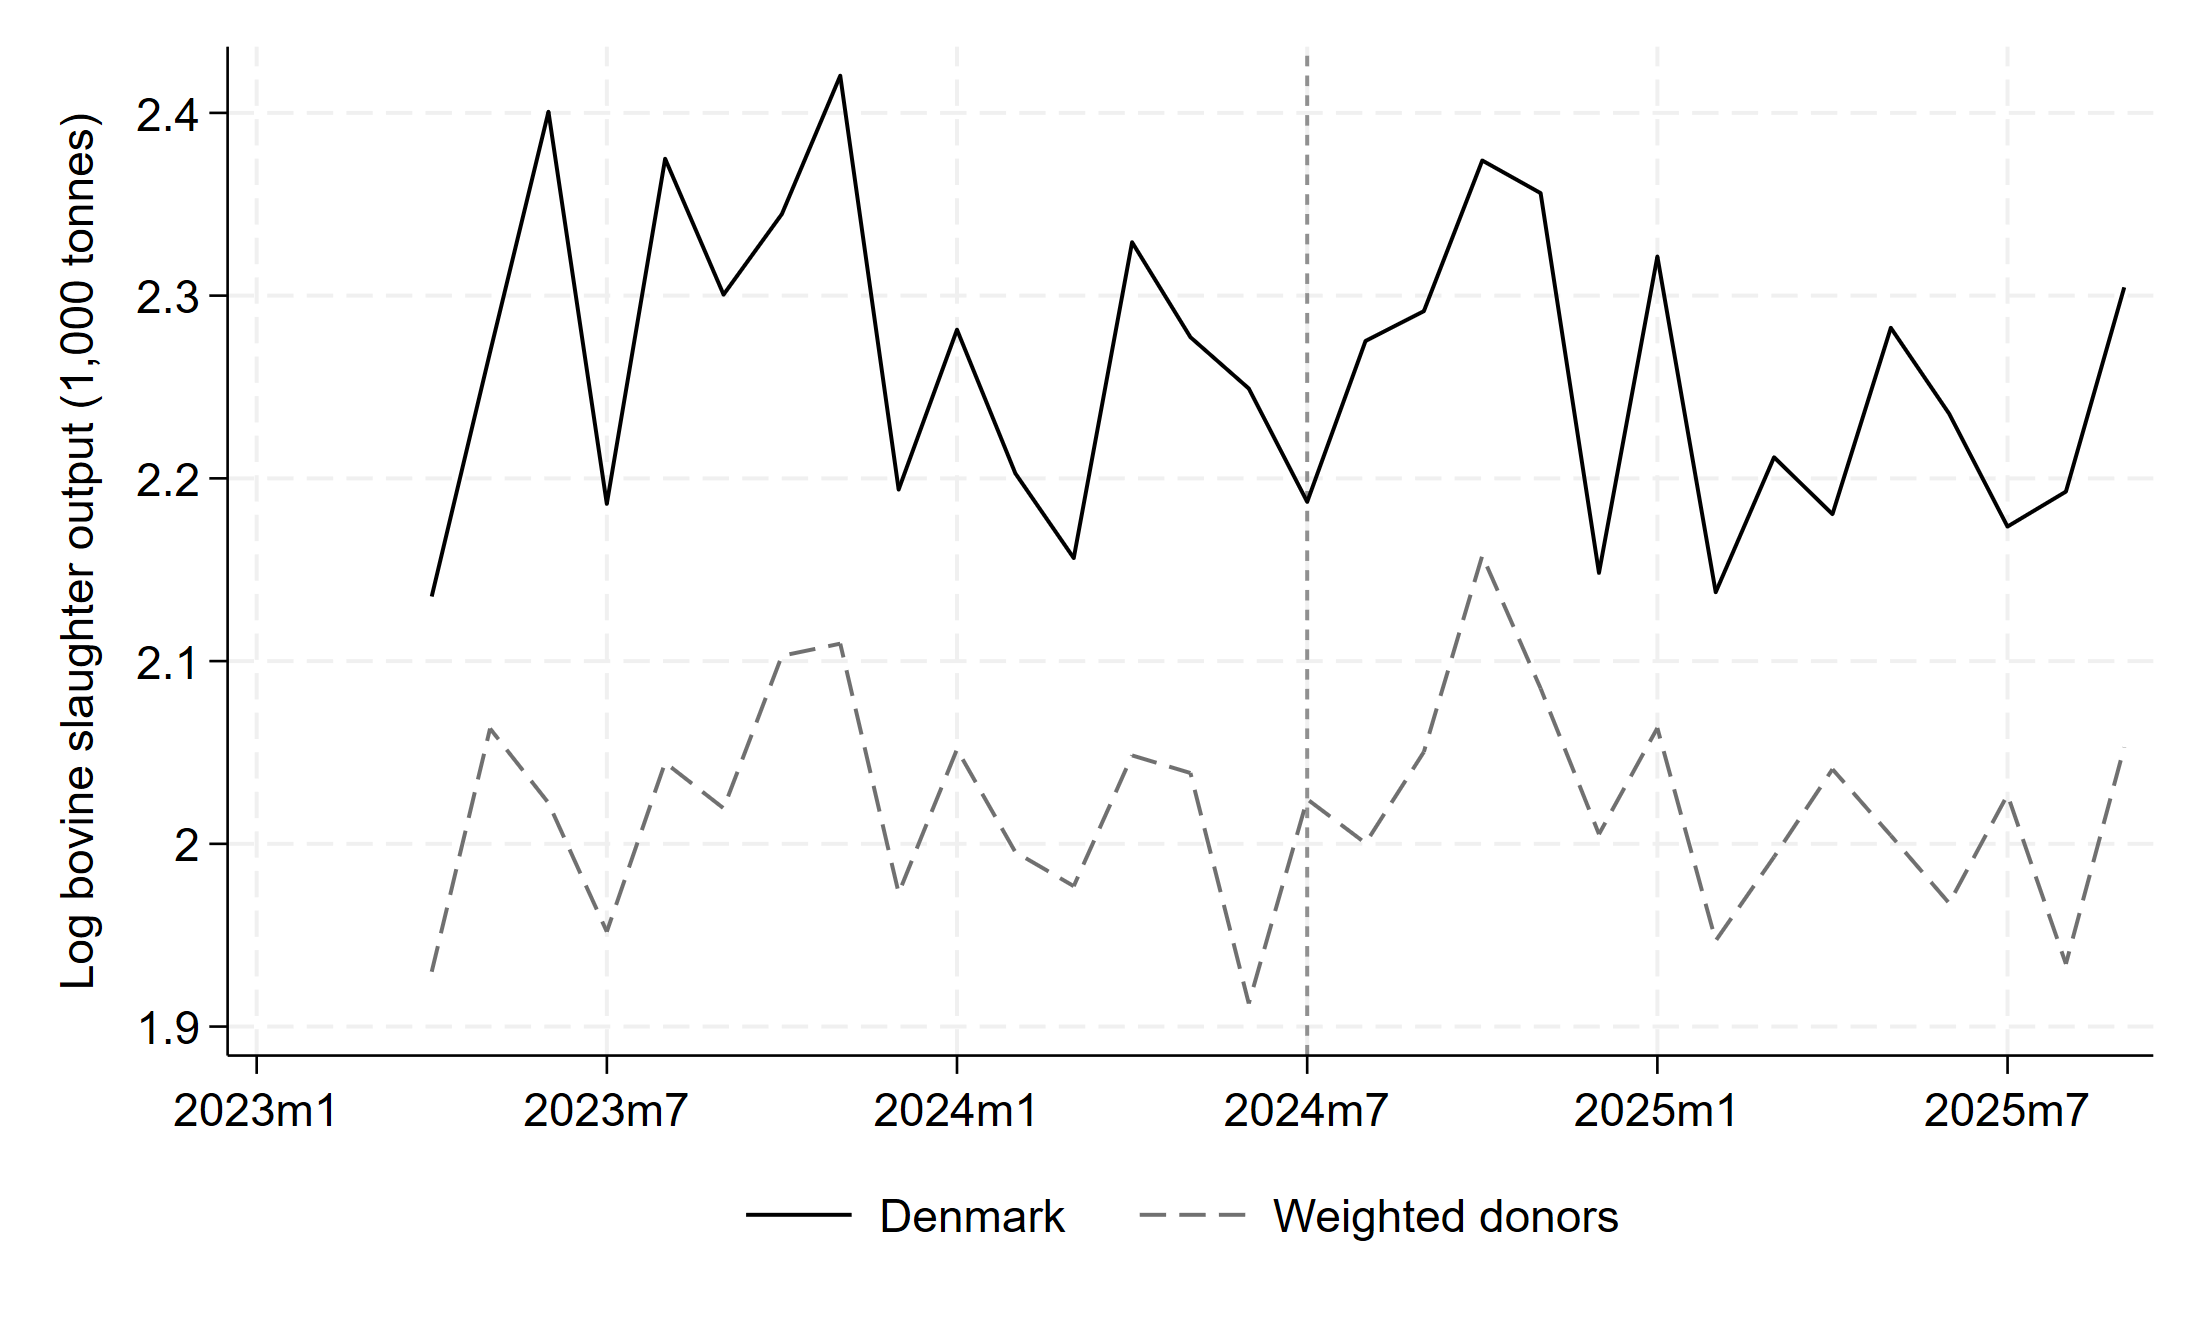
\includegraphics[width=0.9\linewidth]{../outputs/figures/stata/production_sdid.png}
\figurenotes{Eurostat, monthly bovine slaughter weight in thousand tonnes.}{The main sample covers April 2023--September 2025. The dashed vertical line marks July 2024. For display, the donor series is shifted by a constant to match Denmark's pre-treatment mean; this does not change the SDiD estimate. The ATT additionally uses time weights; the plotted level gap alone is not the estimated treatment effect. Production estimates and uncertainty appear in Table~\ref{tab:production}.}
\end{figure}

\subsection{Pre-period support sensitivity}
Table~\ref{tab:window_sensitivity} varies the number of pre-treatment months while holding the July 2024--September 2025 post-period and each outcome's donor set fixed. The slaughter outcomes here remain in raw logs; the seasonally adjusted 54-month specification in Table~\ref{tab:production} is a separate joint sensitivity. Fit is measured on the common April 2023--June 2024 pre-period after removing the mean treated--synthetic gap, as permitted by synthetic DiD's intercept. Longer support slightly improves this in-sample fit for country HICP at 36 and 54 months, while worsening it for the other outcomes. No outcome's preferred window is chosen by another outcome's fit. These point estimates use no-inference diagnostic runs, so the table does not supply new standard errors. In-sample fit cannot establish the untreated post-period path; a prespecified held-out pre-period and donor-weight audit would provide stronger validation.

\begin{table}[htbp]\centering
\caption{Synthetic-DiD window sensitivity by outcome}\label{tab:window_sensitivity}
\small
\begin{tabular}{lrrrr}\toprule
Pre-treatment months & 15 & 24 & 36 & 54 \\\midrule
\multicolumn{5}{l}{\textit{Panel A. Point ATT}} \\
Danish beef versus food CPI & 0.0759 & 0.0427 & 0.0615 & 0.0597 \\
Denmark versus EU beef HICP & 0.0157 & 0.0283 & 0.0231 & 0.0223 \\
Slaughter weight & $-0.0661$ & $-0.0777$ & $-0.0206$ & $-0.0143$ \\
Slaughter heads & $-0.0350$ & $-0.0531$ & $-0.0089$ & $-0.0091$ \\
Extra-EU bilateral imports & $-0.0801$ & $-0.0770$ & $-0.0791$ & $-0.0843$ \\\addlinespace
\multicolumn{5}{l}{\textit{Panel B. Centered pre-gap RMSE on common 15 months}} \\
Danish beef versus food CPI & 0.0054 & 0.0099 & 0.0118 & 0.0111 \\
Denmark versus EU beef HICP & 0.0100 & 0.0102 & 0.0096 & 0.0097 \\
Slaughter weight & 0.0562 & 0.0598 & 0.0622 & 0.0630 \\
Slaughter heads & 0.0562 & 0.0609 & 0.0633 & 0.0640 \\
Extra-EU bilateral imports & 0.0650 & 0.0801 & 0.0861 & 0.0963 \\\bottomrule
\end{tabular}
\figurenotes{Statistics Denmark, Eurostat, and European Commission data.}{All specifications retain their respective published donor sets. The 15-, 24-, 36-, and 54-month pre-periods all end in June 2024. ATT values are Stata no-inference diagnostics; Panel B evaluates every fit on the same April 2023--June 2024 months and permits a constant gap. Slaughter entries do not remove seasonality. The extra-EU outcome is log(1+tonnes), not total imports.}
\end{table}

\clearpage
\subsection{Additional price and trade comparisons}
\begin{figure}[htbp]\centering
\caption{Official-data synthetic DiD: beef and weighted donors}\label{fig:b_sdid}
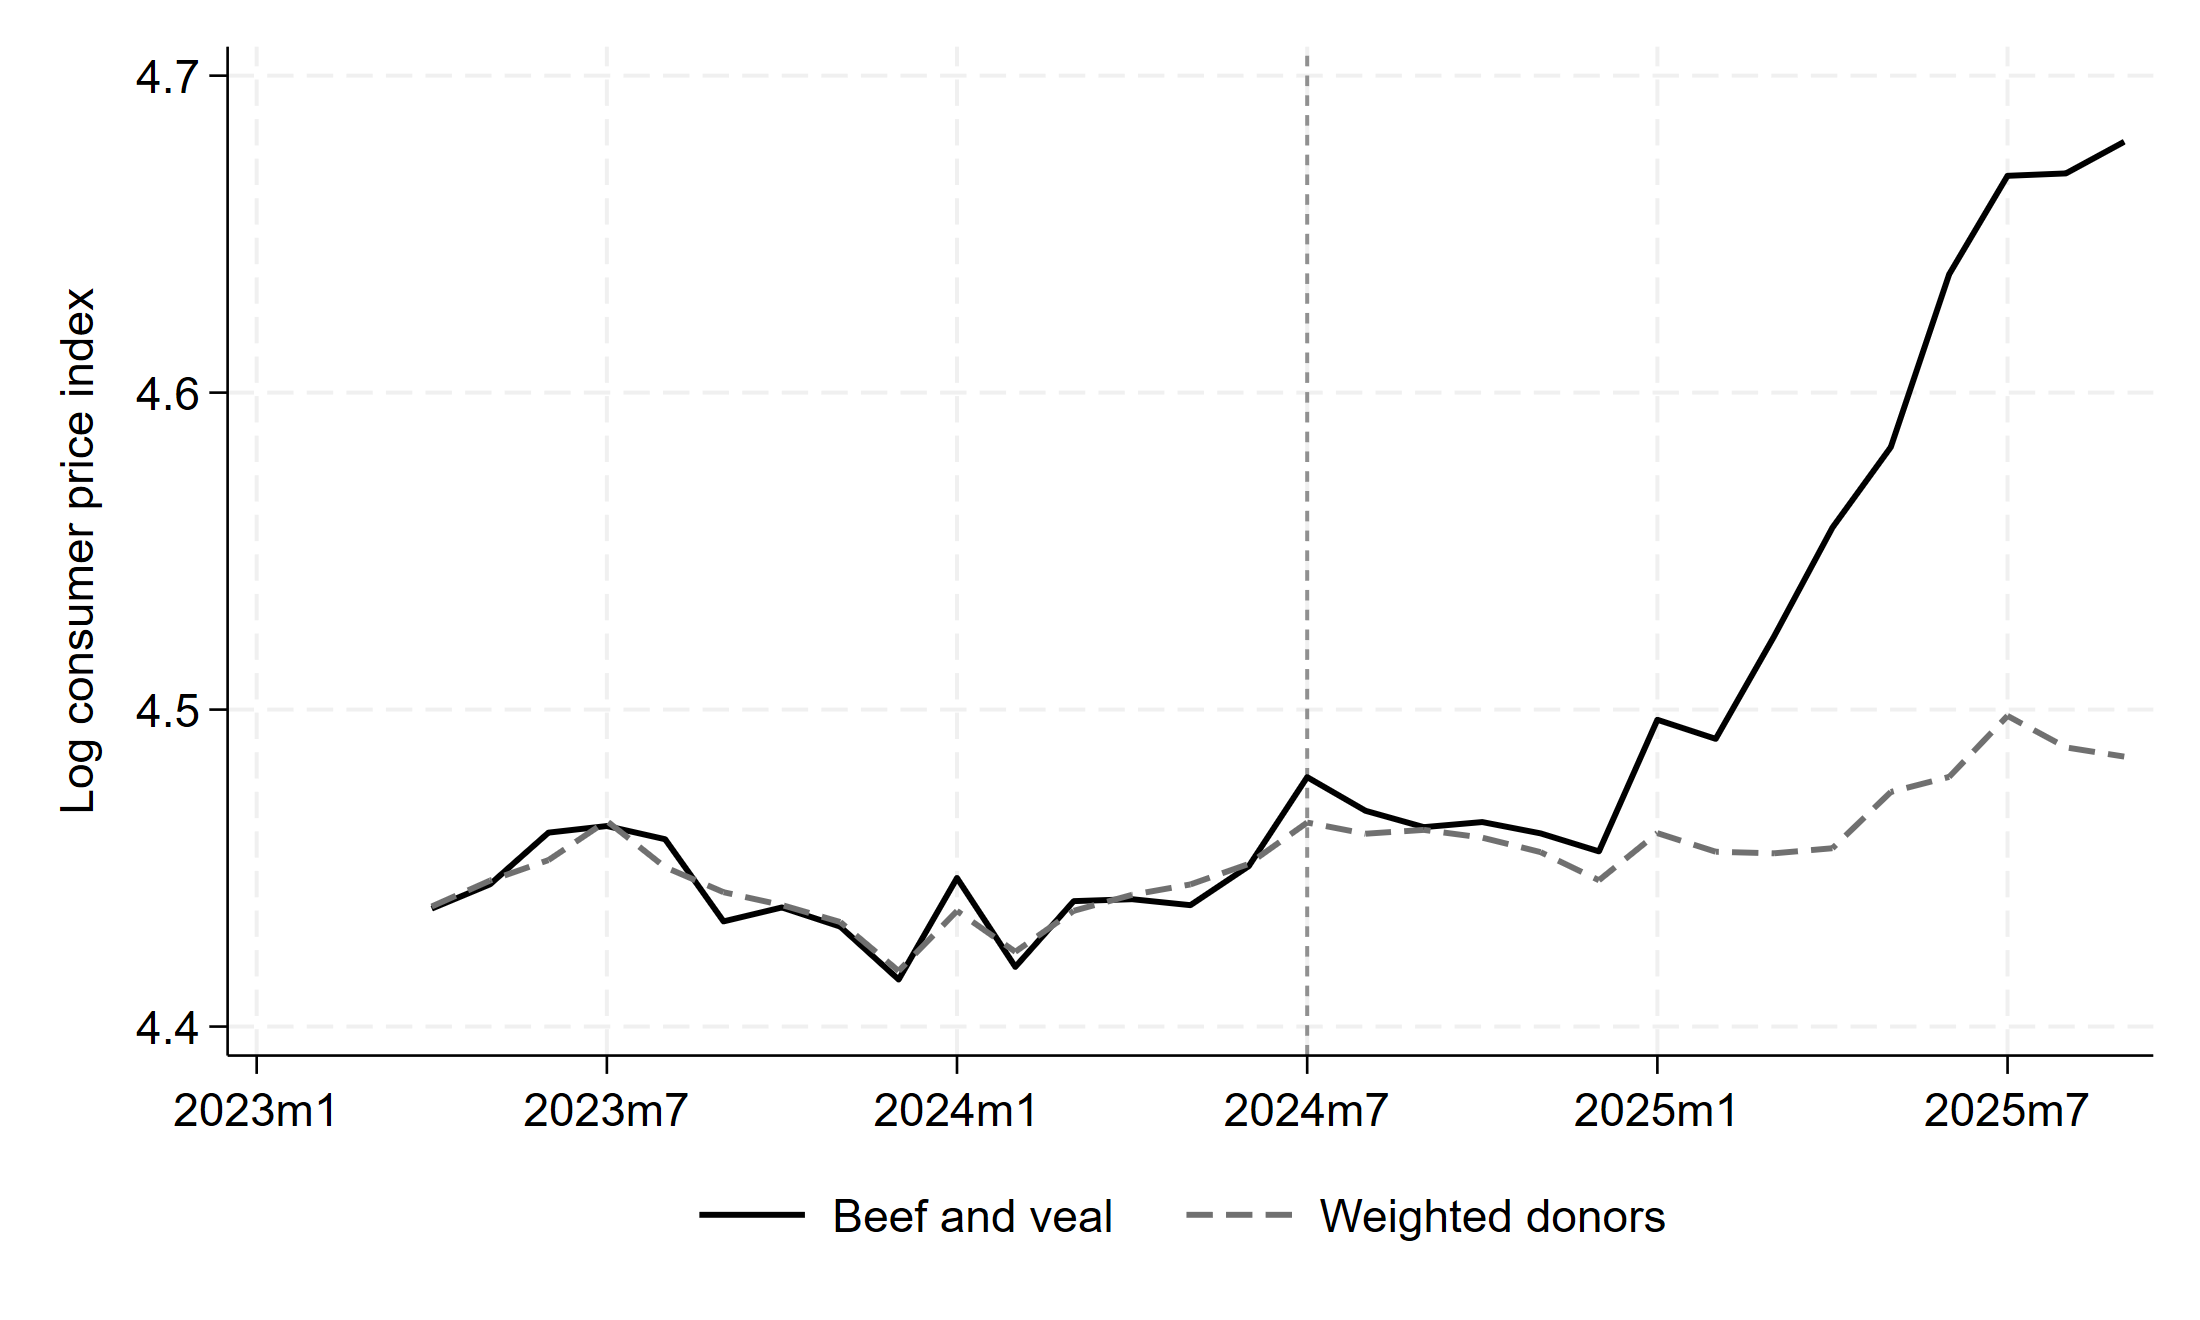
\includegraphics[width=0.9\linewidth]{../outputs/figures/stata/aggregate_sdid.png}
\figurenotes{Statistics Denmark.}{Series are log CPI for beef and veal and the SDiD-weighted donor series over the symmetric 15-month pre/post window. The dashed vertical line marks July 2024, the first post-announcement month. For display, the donor series is shifted by a constant to match the treated series' pre-treatment mean; this does not change the SDiD estimate.}\end{figure}

\begin{figure}[htbp]\centering
\caption{Country-level synthetic DiD: Danish beef-and-veal consumer prices}\label{fig:b_country_sdid}
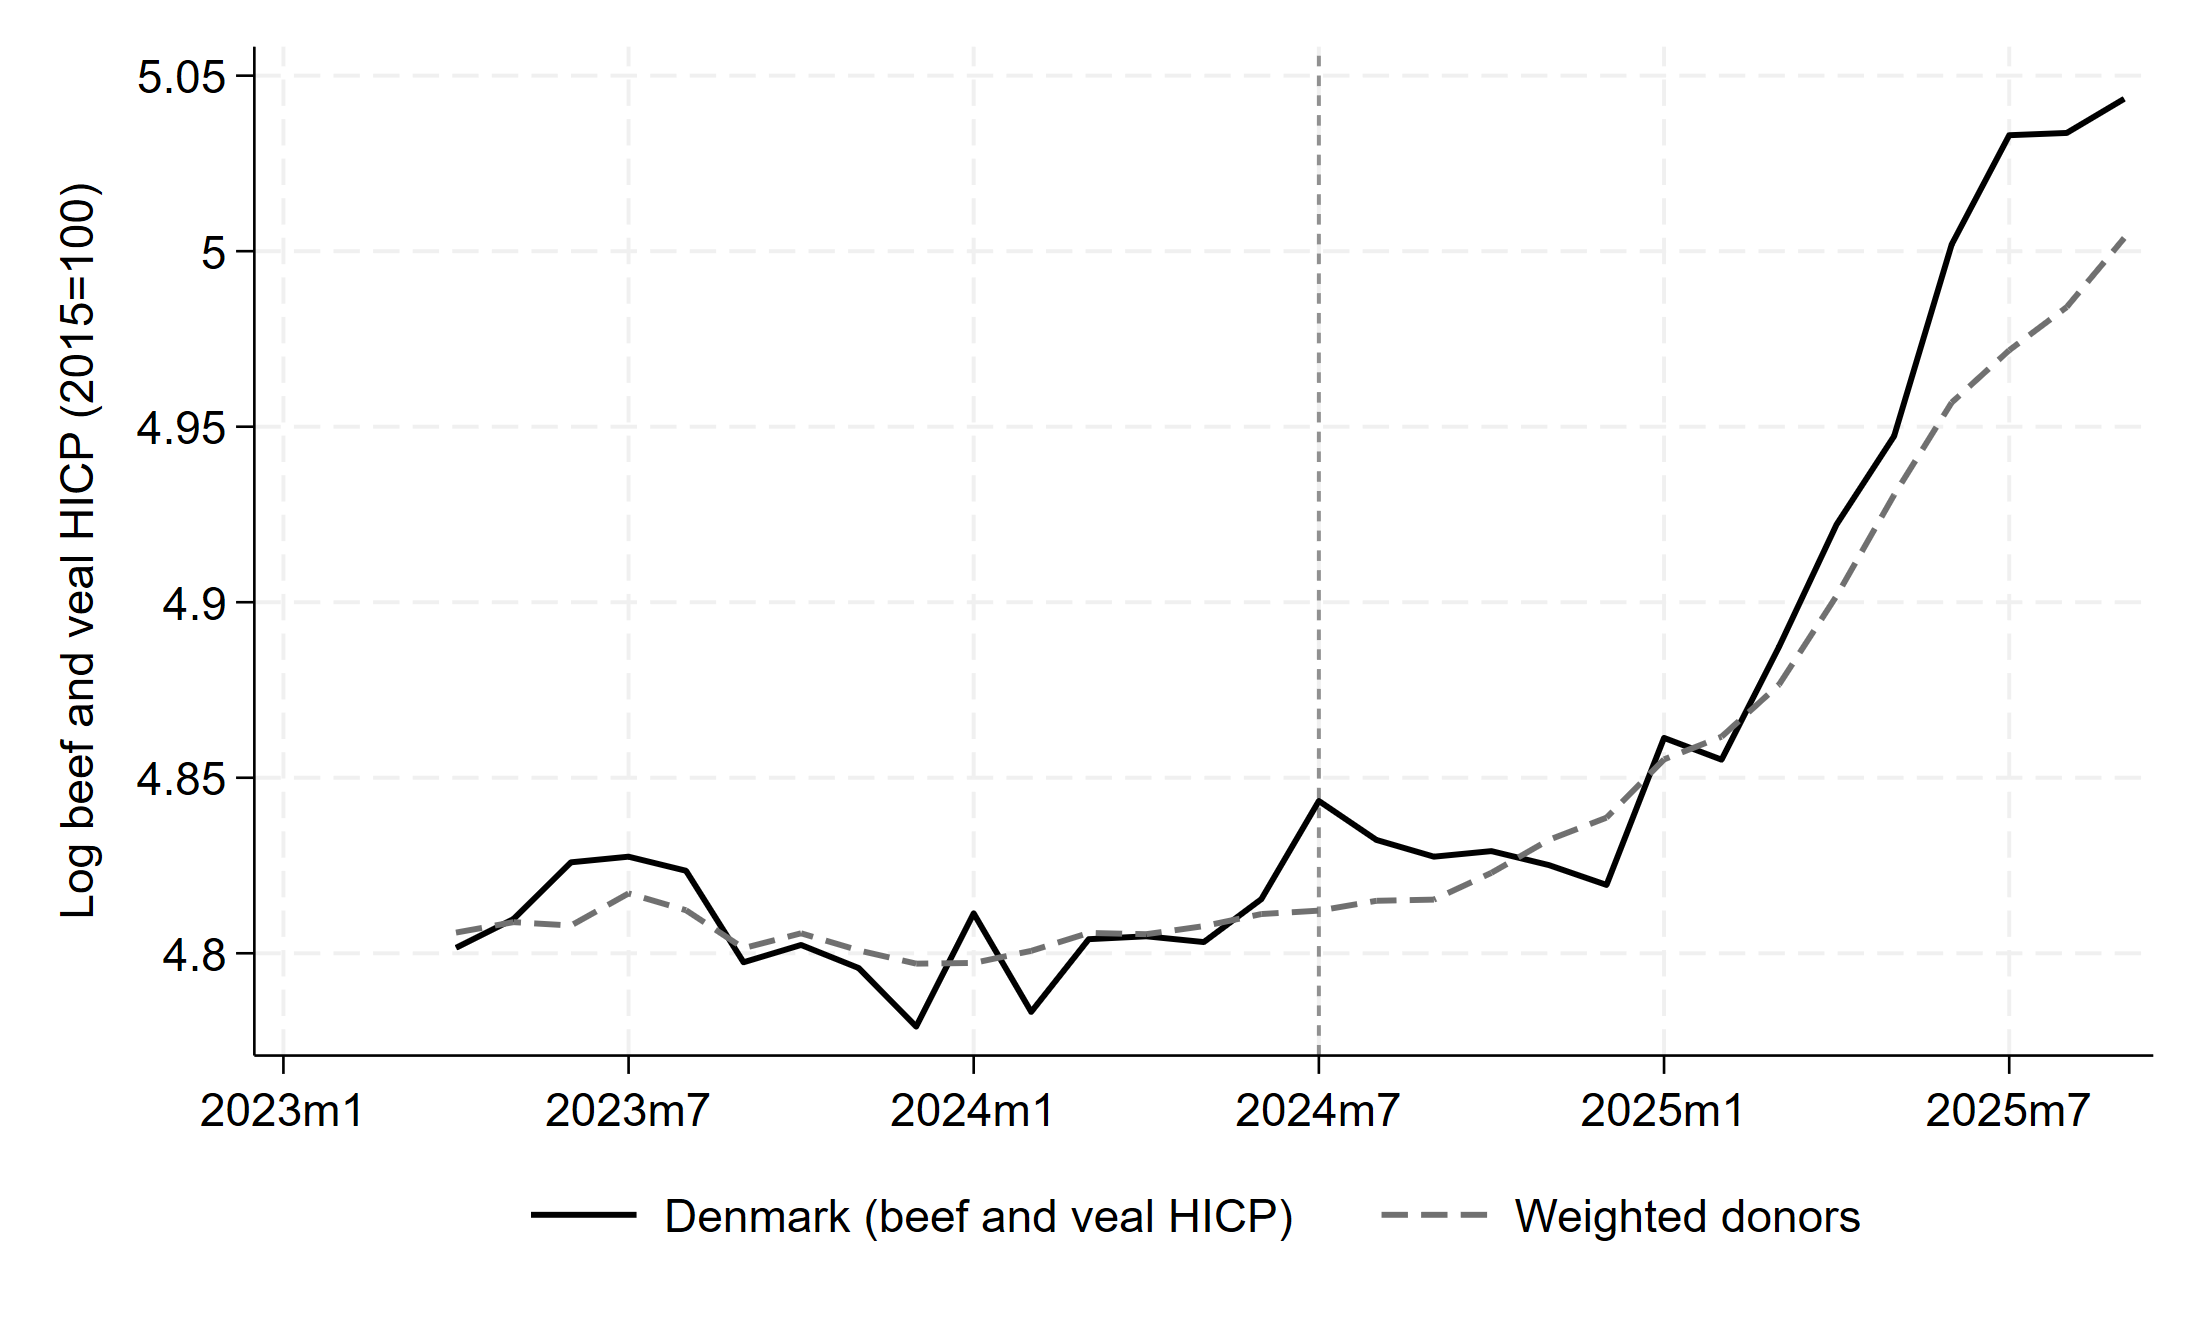
\includegraphics[width=0.9\linewidth]{../outputs/figures/stata/country_sdid.png}
\figurenotes{Eurostat, Harmonised Index of Consumer Prices; national statistical institutes.}{Series are log beef-and-veal HICP for Denmark and the SDiD-weighted donor series constructed from the other 26 EU Member States over April 2023--September 2025. The panel contains 810 observations, with 15 pre-treatment and 15 post-treatment months. The dashed line marks July 2024. The ATT is 0.0157 (placebo standard error 0.0293; $p=0.593$; 95 percent interval $[-0.0417,0.0731]$; 200 replications). For display, the donor series is shifted by a constant to match Denmark's pre-treatment mean; this does not change the SDiD estimate. The pre-treatment centered-gap root-mean-square error is 0.0100 log points. The Danish HICP is compiled by Statistics Denmark; the exercise tests an alternative control group.}\end{figure}

\begin{figure}[htbp]\centering
\caption{Synthetic DiD: beef imports into Denmark}\label{fig:b_trade_sdid}
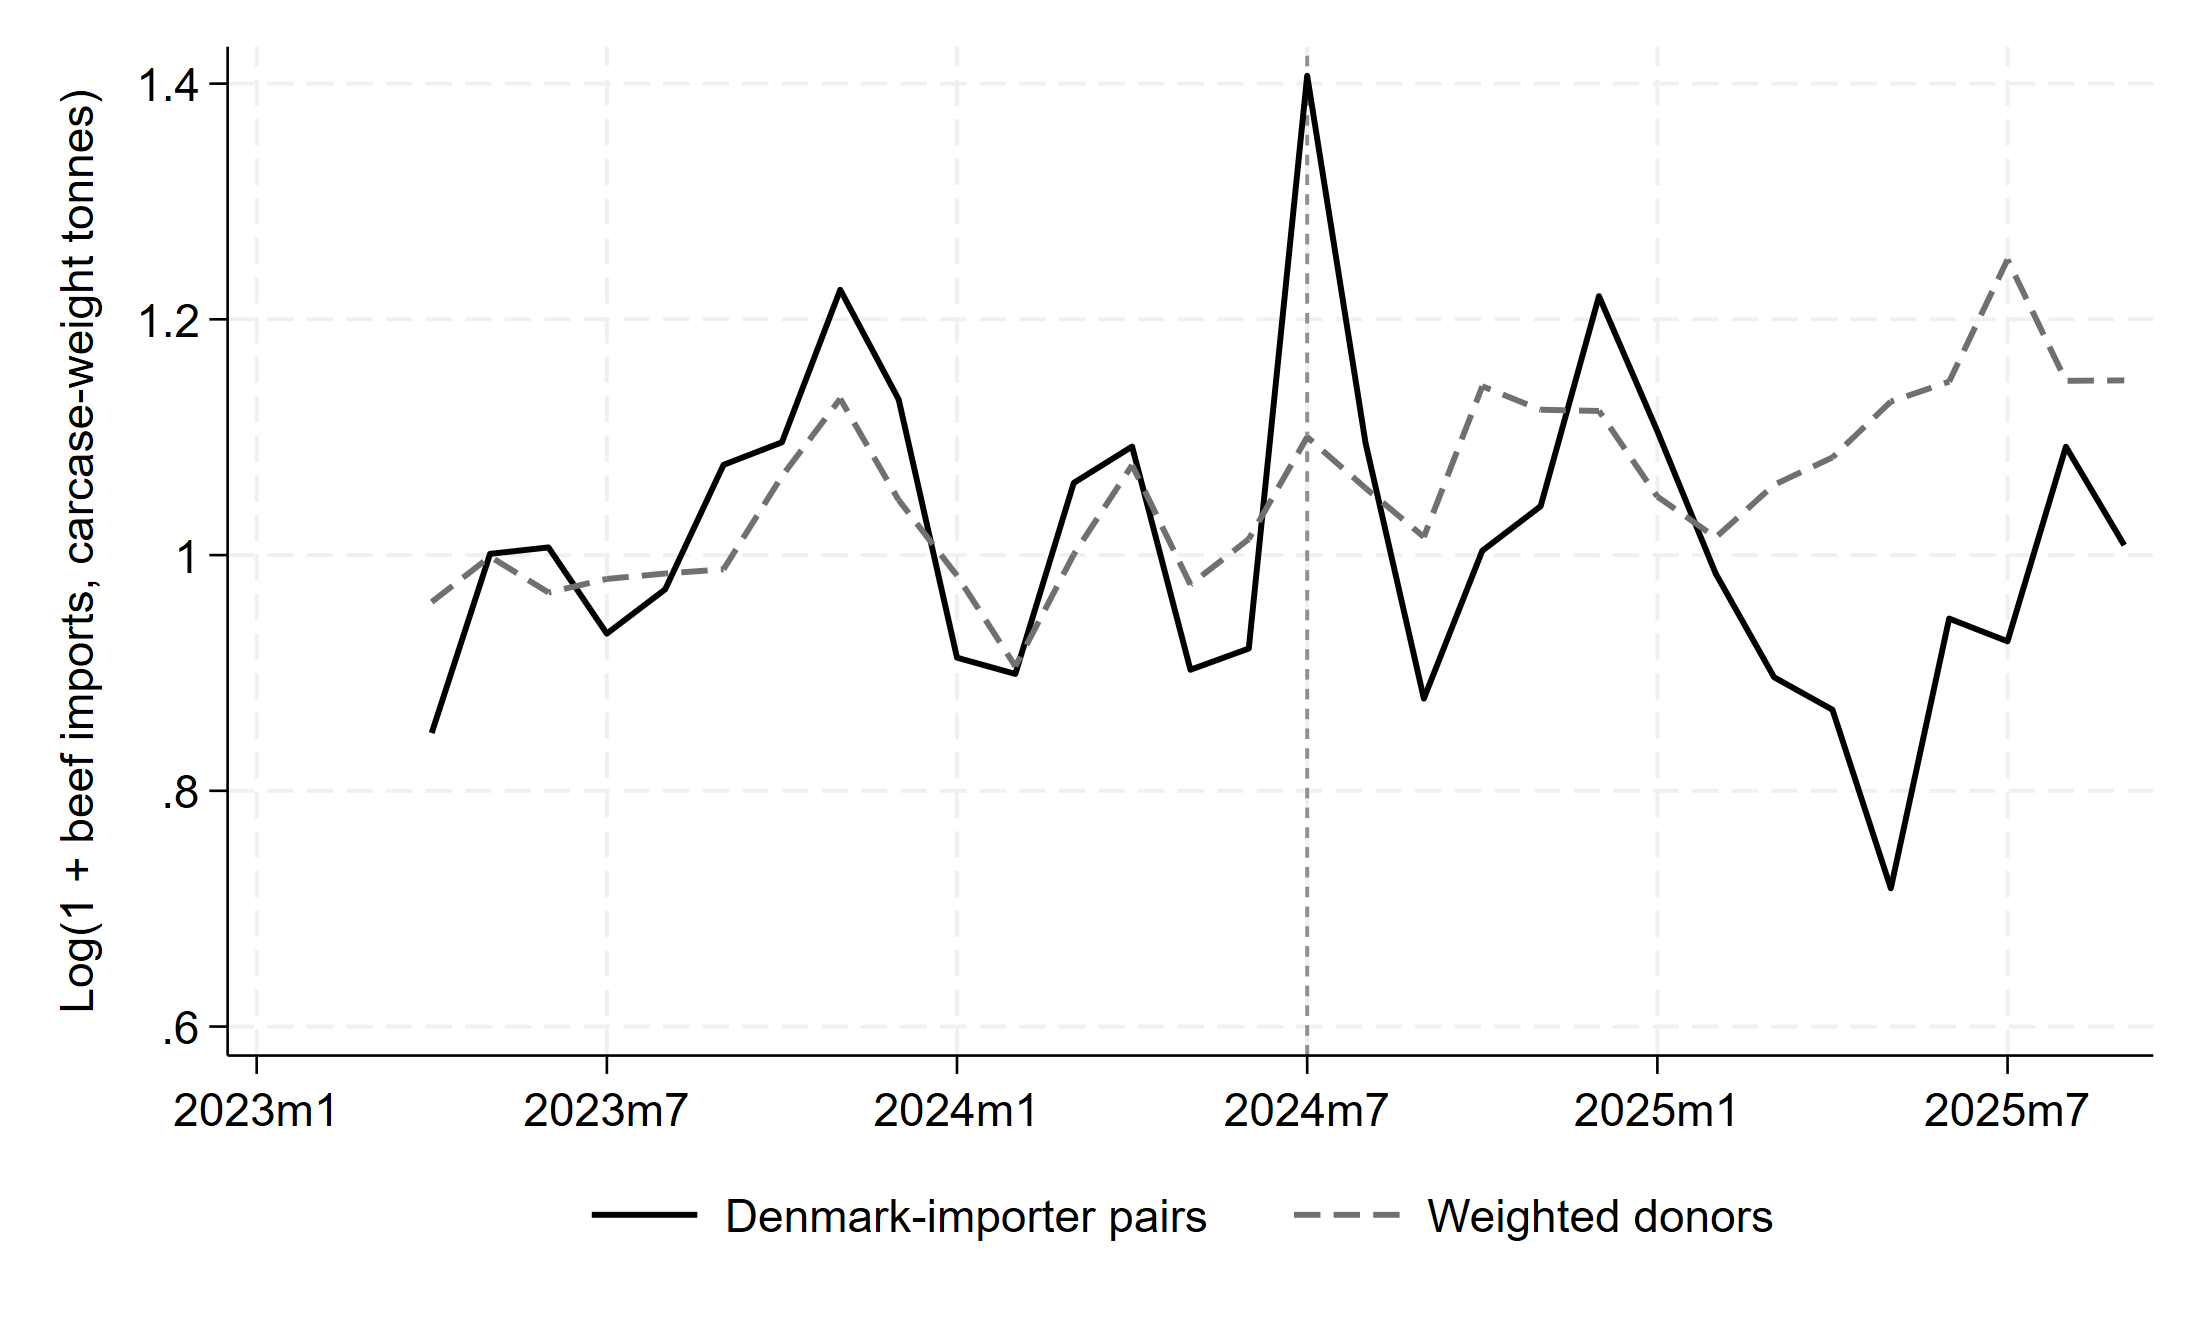
\includegraphics[width=0.9\linewidth]{../outputs/figures/stata/beef_trade_pair_sdid.png}
\figurenotes{European Commission, Beef Trade Data Explorer; Eurostat COMEXT.}{Series are mean log-one-plus monthly extra-EU beef imports, measured in carcass-weight tonnes, for Denmark--partner pairs and their SDiD-weighted donor series over the symmetric April 2023--September 2025 window. The dashed vertical line marks July 2024. The ATT is $-0.0801$ (unit-cluster bootstrap standard error 0.0782; $p=0.306$; 200 replications). For display, the donor series is shifted by a constant to match the treated series' pre-treatment mean; this does not change the SDiD estimate.}\end{figure}
\end{document}
